%% whole_genome_alignment.tex
%% Author: Leighton Pritchard
%% Copyright: James Hutton Institute
%% A brief description of whole genome alignment and comparison


% SUBSECTION: Whole genome alignments
\subsection{An Introduction to Pairwise Genome Alignment}

% What do you align, and why?
\begin{frame}
  \frametitle{What to align, and why?}
  To be useful, aligned genomes should:
  \begin{itemize}
    \item derive from a sufficiently recent common ancestor, so homologous regions can be identified
    \item derive from a sufficiently distant common ancestor, so that there are ``interesting'' differences to be identified
    \item \textbf{help to answer your biological question}: is your question organism or phenotype-specific? 
  \end{itemize}
  \begin{center}
    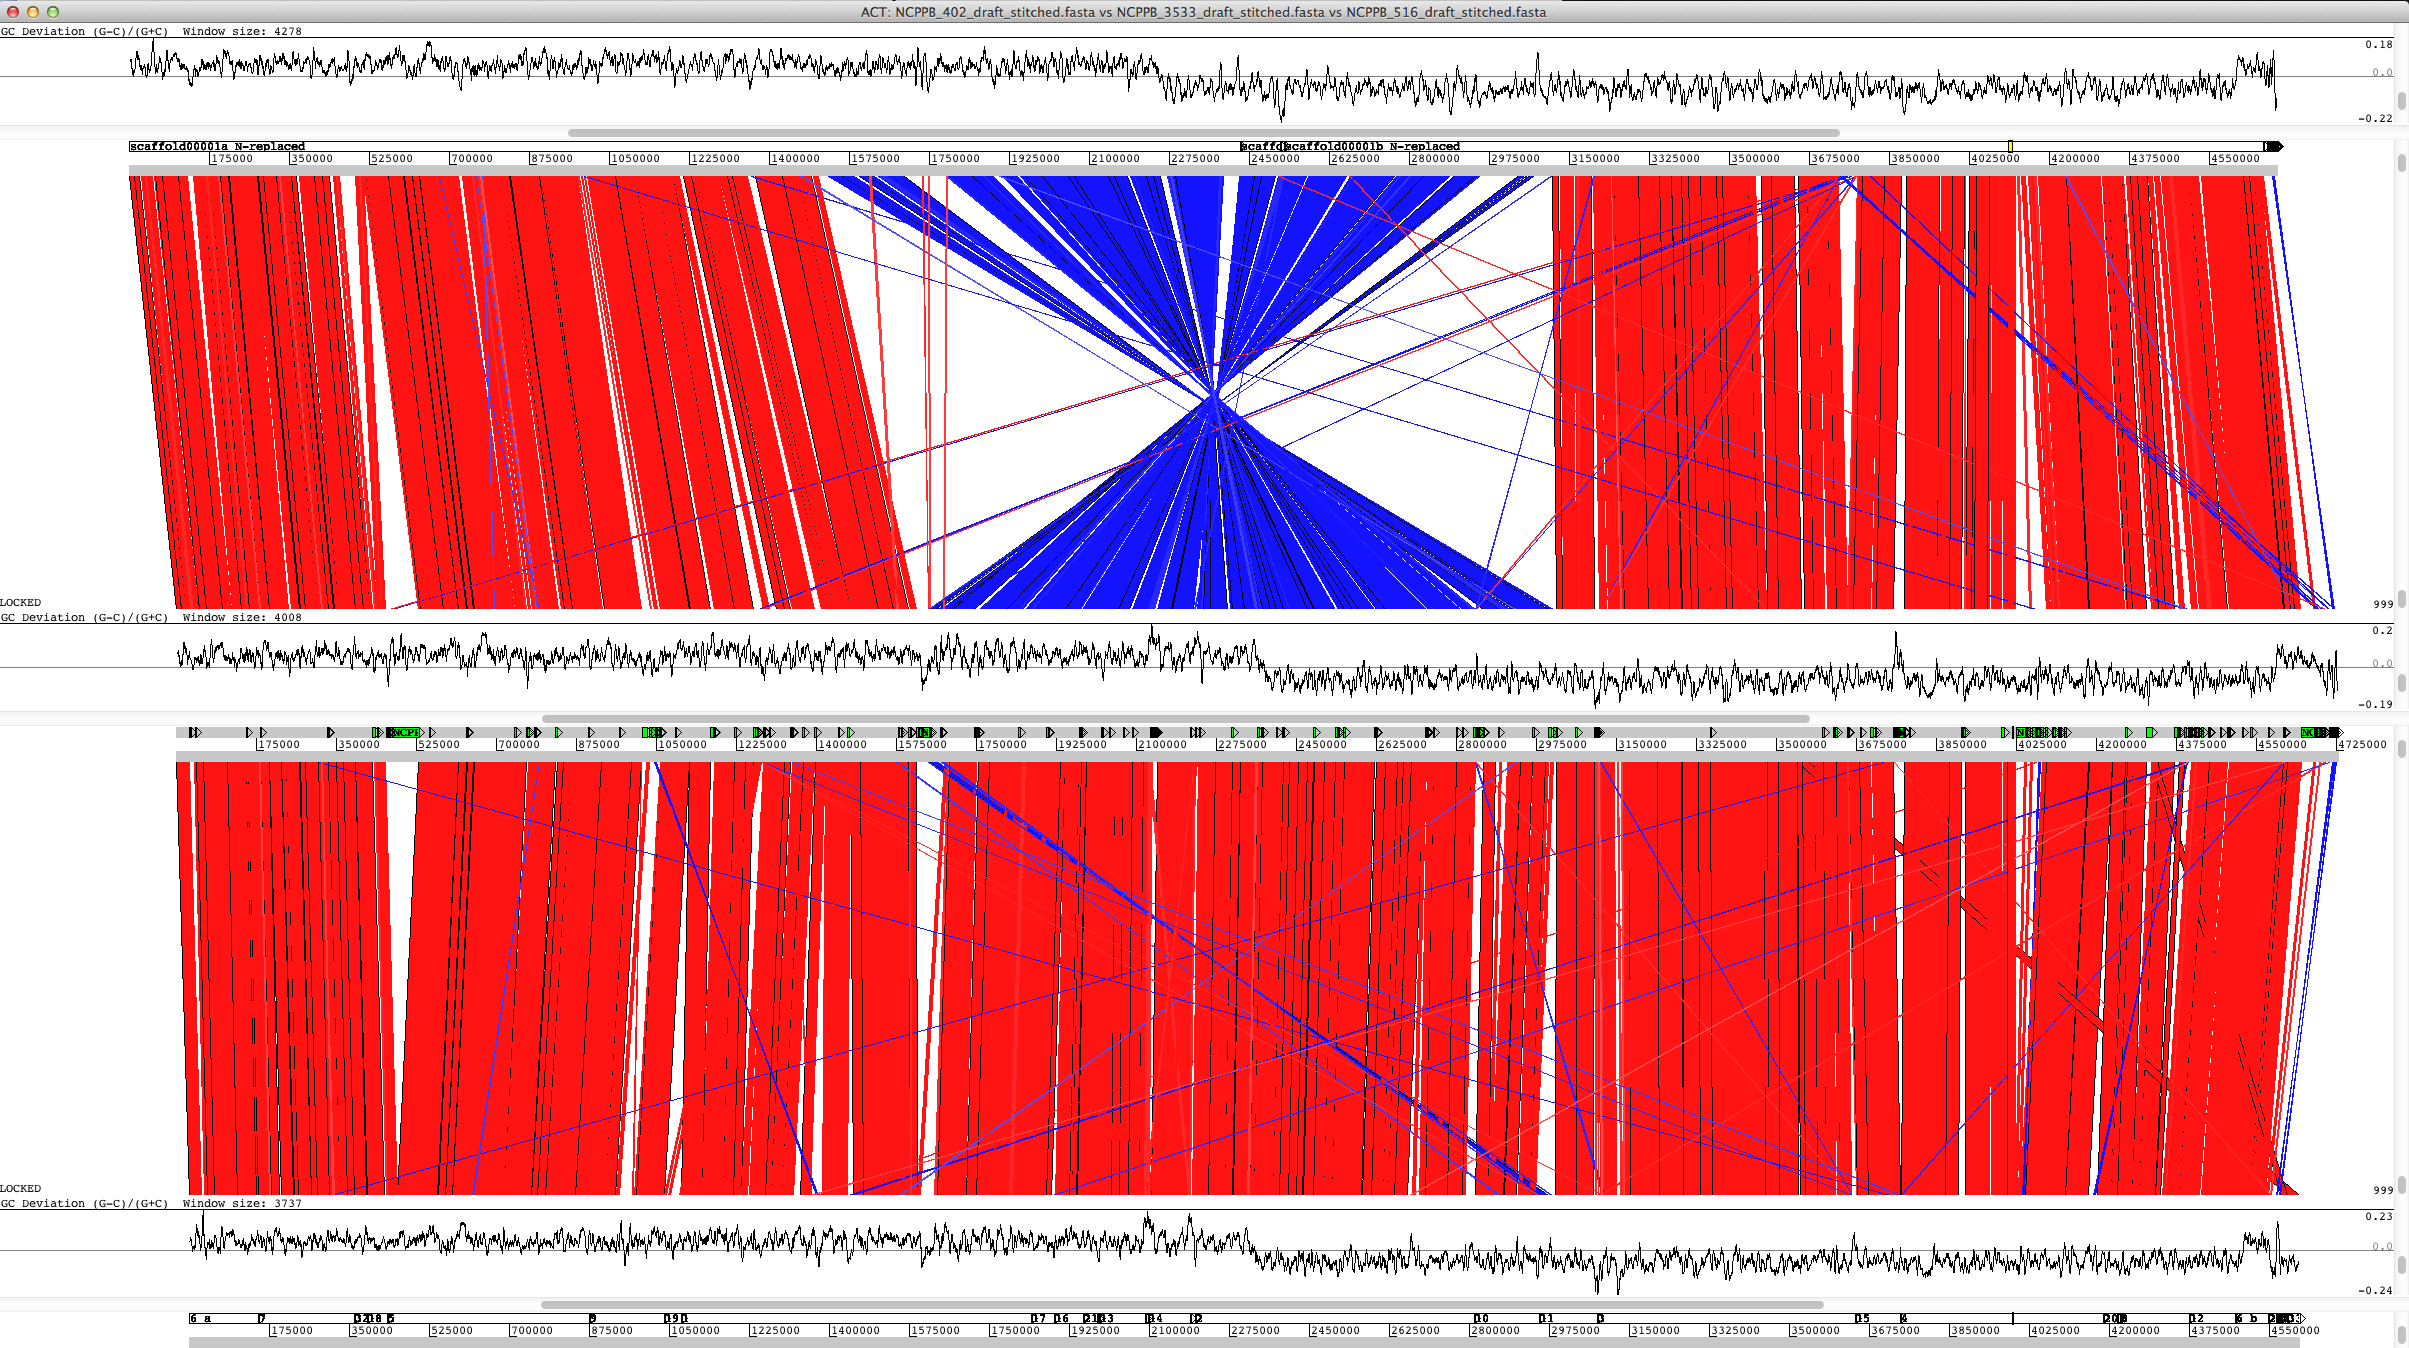
\includegraphics[width=0.6\textwidth]{images/act_comparison}
  \end{center}  
\end{frame}

% How do you align, and why?
\begin{frame}
  \frametitle{How to align, and why?}
  Naive sequence aligners (Needleman-Wunsch, Smith-Waterman) are not appropriate for genome alignment
  \begin{itemize}
    \item Computationally expensive on large sequences
    \item Cannot handle rearrangements
  \end{itemize}
  Very many alternative alignment algorithms proposed
  \begin{itemize}
    \item \textbf{megaBLAST} {\tiny\href{http://www.ncbi.nlm.nih.gov/blast/html/megablast.html}{http://www.ncbi.nlm.nih.gov/blast/html/megablast.html}}
    \item \textbf{MUMmer} {\tiny\href{http://mummer.sourceforge.net/}{http://mummer.sourceforge.net/}}
    \item BLAT {\tiny\href{http://genome.ucsc.edu/goldenPath/help/blatSpec.html}{http://genome.ucsc.edu/goldenPath/help/blatSpec.html}}
    \item LASTZ {\tiny\href{http://www.bx.psu.edu/~rsharris/lastz/}{http://www.bx.psu.edu/$\sim$rsharris/lastz/}}
    \item LAGAN {\tiny\href{http://lagan.stanford.edu/lagan_web/index.shtml}{http://lagan.stanford.edu/lagan\_web/index.shtml}}
    \item and many, many more$\ldots$        
  \end{itemize}
  Example exercises in \url{data/whole_genome_alignment}.
\end{frame}

% megaBLAST
\begin{frame}
  \frametitle{megaBLAST}
  Optimised for speed, over BLASTN\footnote{\tiny{\href{http://www.ncbi.nlm.nih.gov/blast/Why.shtml}{http://www.ncbi.nlm.nih.gov/blast/Why.shtml}}}
  \begin{itemize}
    \item Genome-level searches
    \item Queries on large sequence sets
    \item Long alignments of very similar sequence
  \end{itemize}
  Uses the greedy algorithm by Zhang \textit{et al.}\footnote{\tiny{\href{http://dx.doi.org/10.1089/10665270050081478}{Zhang \textit{et al}. (2000) \textit{J. Comp. Biol.} \textbf{7}:203-214 doi:10.1089/10665270050081478}}}, \textbf{not} BLAST algorithm.
  \begin{itemize}
    \item Concatenates queries (``query packing'') to improve performance
    \item Two modes: \textbf{megaBLAST} and discontinuous (\textbf{dc-megablast}) for divergent sequences
  \end{itemize}
  BLASTN now uses the megaBLAST algorithm by default
\end{frame}

% BLAST vs megaBLAST
\begin{frame}
  \frametitle{BLAST vs megaBLAST}
  megaBLAST is faster, but does it matter for biology?\\[0.2cm]
  BLAST (top) and megaBLAST (bottom) pairwise comparisons:
  \begin{center}
    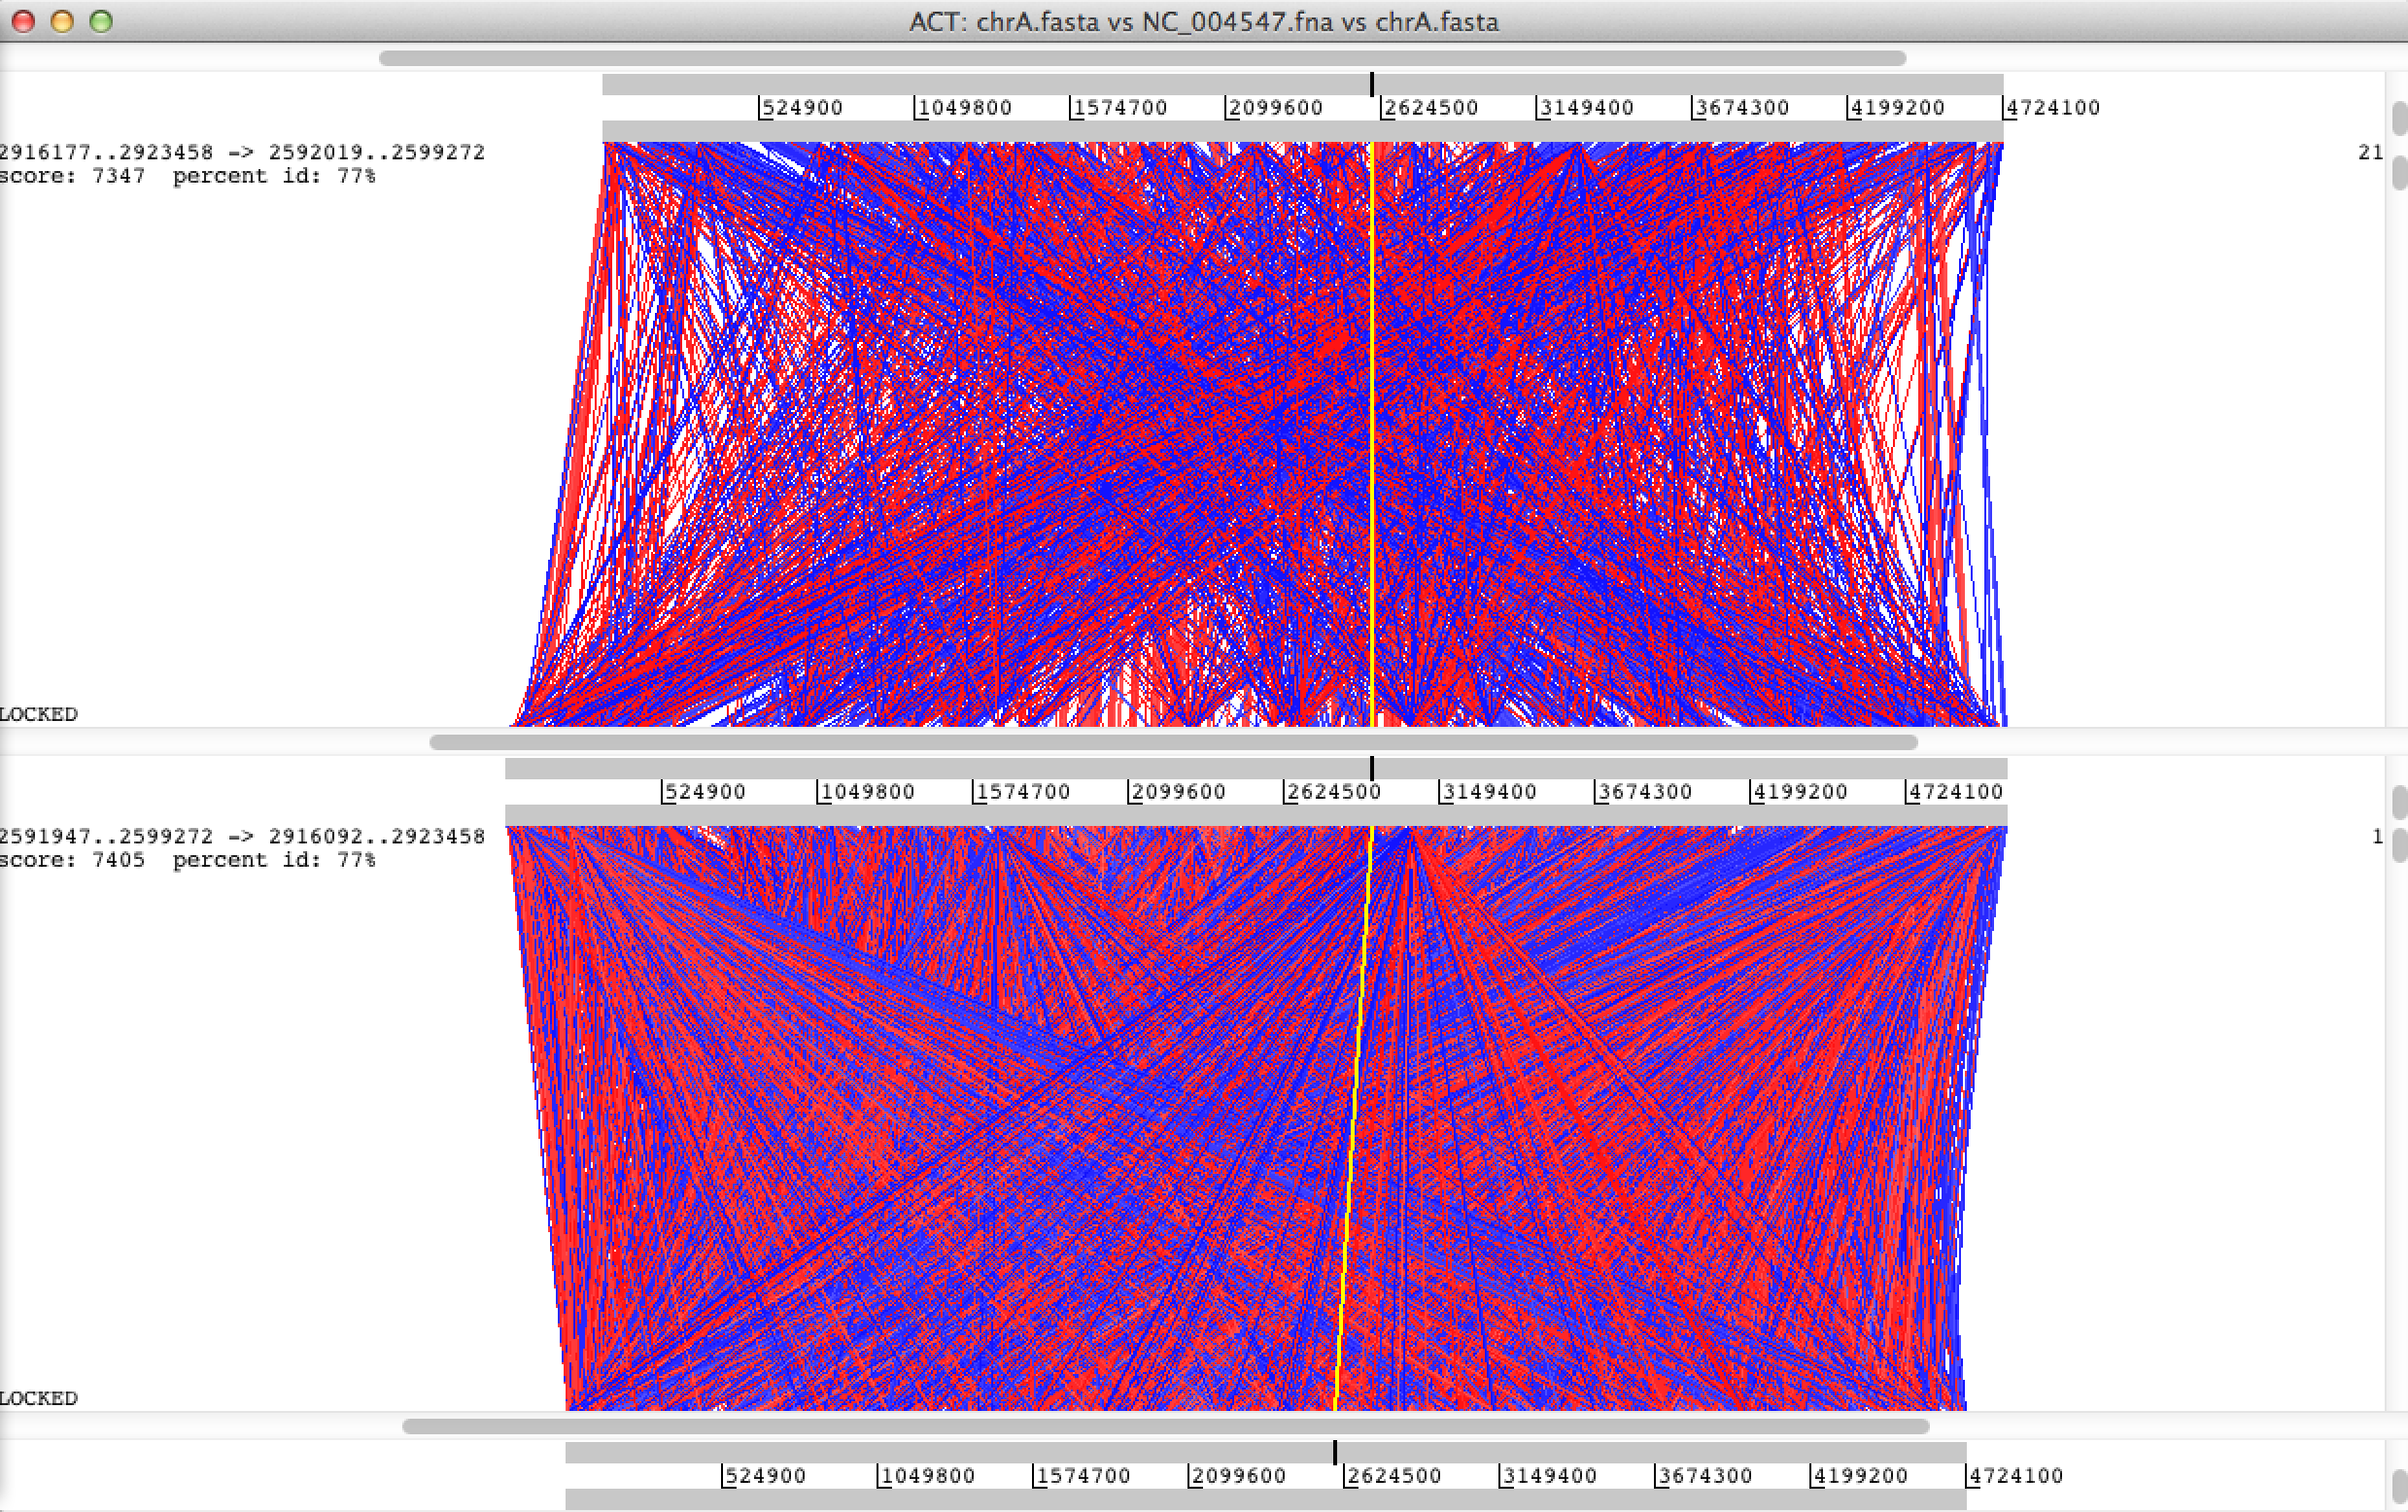
\includegraphics[width=0.8\textwidth]{images/act_wgs6}
  \end{center}    
\end{frame}

% BLAST vs megaBLAST
\begin{frame}
  \frametitle{BLAST vs megaBLAST}
  Filter out weak matches - not quite identical:
  \begin{center}
    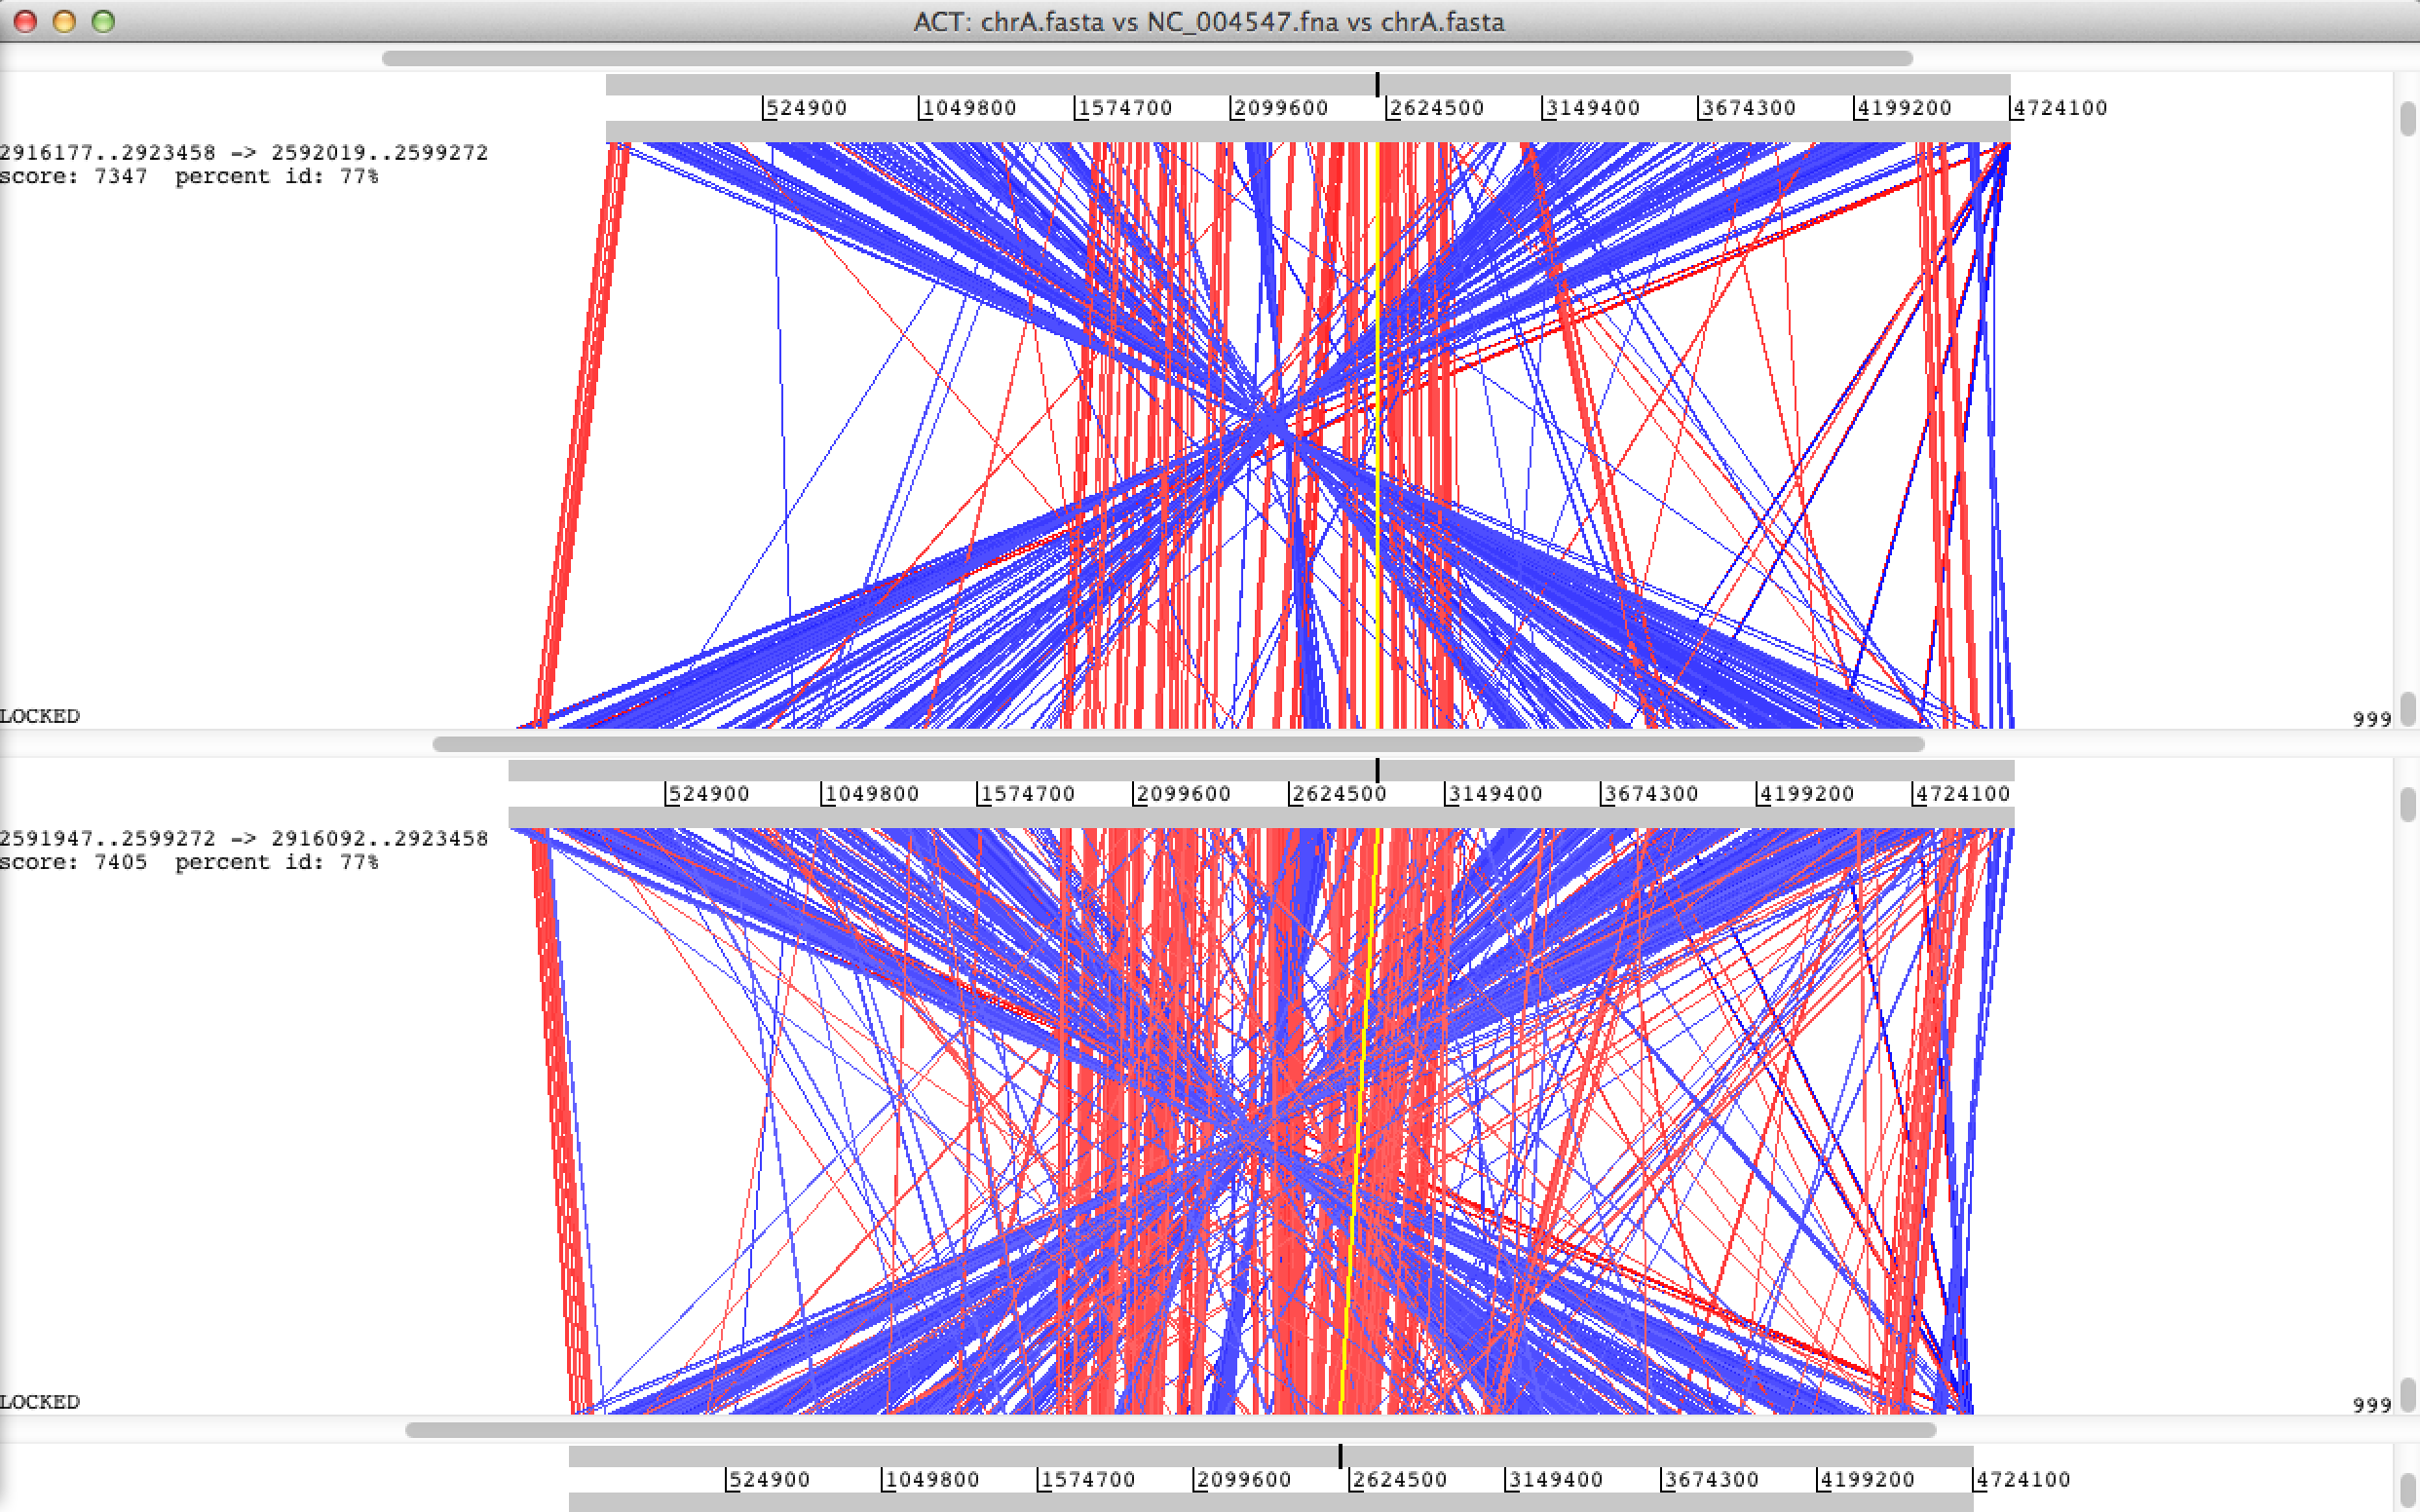
\includegraphics[width=0.9\textwidth]{images/act_wgs7}
  \end{center}    
\end{frame}

% MUMmer implements suffix trees
\begin{frame}
  \frametitle{MUMmer\footnote{\tiny{\href{http://dx.doi.org/10.1186/gb-2004-5-2-r12}{Kurtz \textit{et al}. (2004) \textit{Genome. Biol.} \textbf{5}:R12 doi:10.1186/gb-2004-5-2-r12}}}}
  Uses \textit{suffix trees} for pattern matching: very fast even for large sequences
  \begin{columns}[T]
    \begin{column}{5cm}  
      \begin{itemize}
        \item Finds \textit{maximal exact matches}
        \item Memory use depends only on the reference sequence size
      \end{itemize}
      Suffix trees: {\tiny(\href{http://en.wikipedia.org/wiki/Suffix_tree}{http://en.wikipedia.org/wiki/Suffix\_tree})}
      \begin{itemize}
        \item Can be built and searched in $O(n)$ time
        \item But useful algorithms are nontrivial
      \end{itemize}
    \end{column}
    \begin{column}{5cm}
      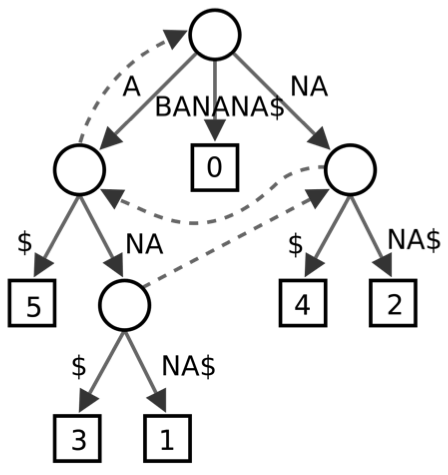
\includegraphics[width=1\textwidth]{images/suffix_tree}
    \end{column}
  \end{columns}      
\end{frame}

% MUMmer algorithm
\begin{frame}
  \frametitle{The MUMmer algorithm\footnote{\tiny{\href{http://dx.doi.org/10.1186/gb-2004-5-2-r12}{Kurtz \textit{et al}. (2004) \textit{Genome. Biol.} \textbf{5}:R12 doi:10.1186/gb-2004-5-2-r12}}}}
  \begin{enumerate}
    \item Identify a non-overlapping subset of maximal exact matches: often \textit{Maximal Unique Matches (MUMs)}
    \item Cluster into \textit{alignment anchors}
    \item Extend between anchors to produce the final alignment
  \end{enumerate}
  This is the basis of a very flexible suite of programs that align different kinds of sequence: \texttt{mummer}, \texttt{nucmer}, \texttt{promer}
  \begin{itemize}
    \item nucleotide and (more sensitive) ``conceptual protein'' alignments
    \item used for genome comparisons, assembly scaffolding, repeat detection, $\ldots$
    \item the basis of other aligners/assemblers (e.g. Mugsy, AMOS)
  \end{itemize}
\end{frame}

% MUMmer vs megaBLAST
\begin{frame}
  \frametitle{MUMmer vs megaBLAST}
  MUMmer identifies fewer weak matches\\[0.2cm]
  megaBLAST (top) and MUMmer (bottom) pairwise comparisons:
  \begin{center}
    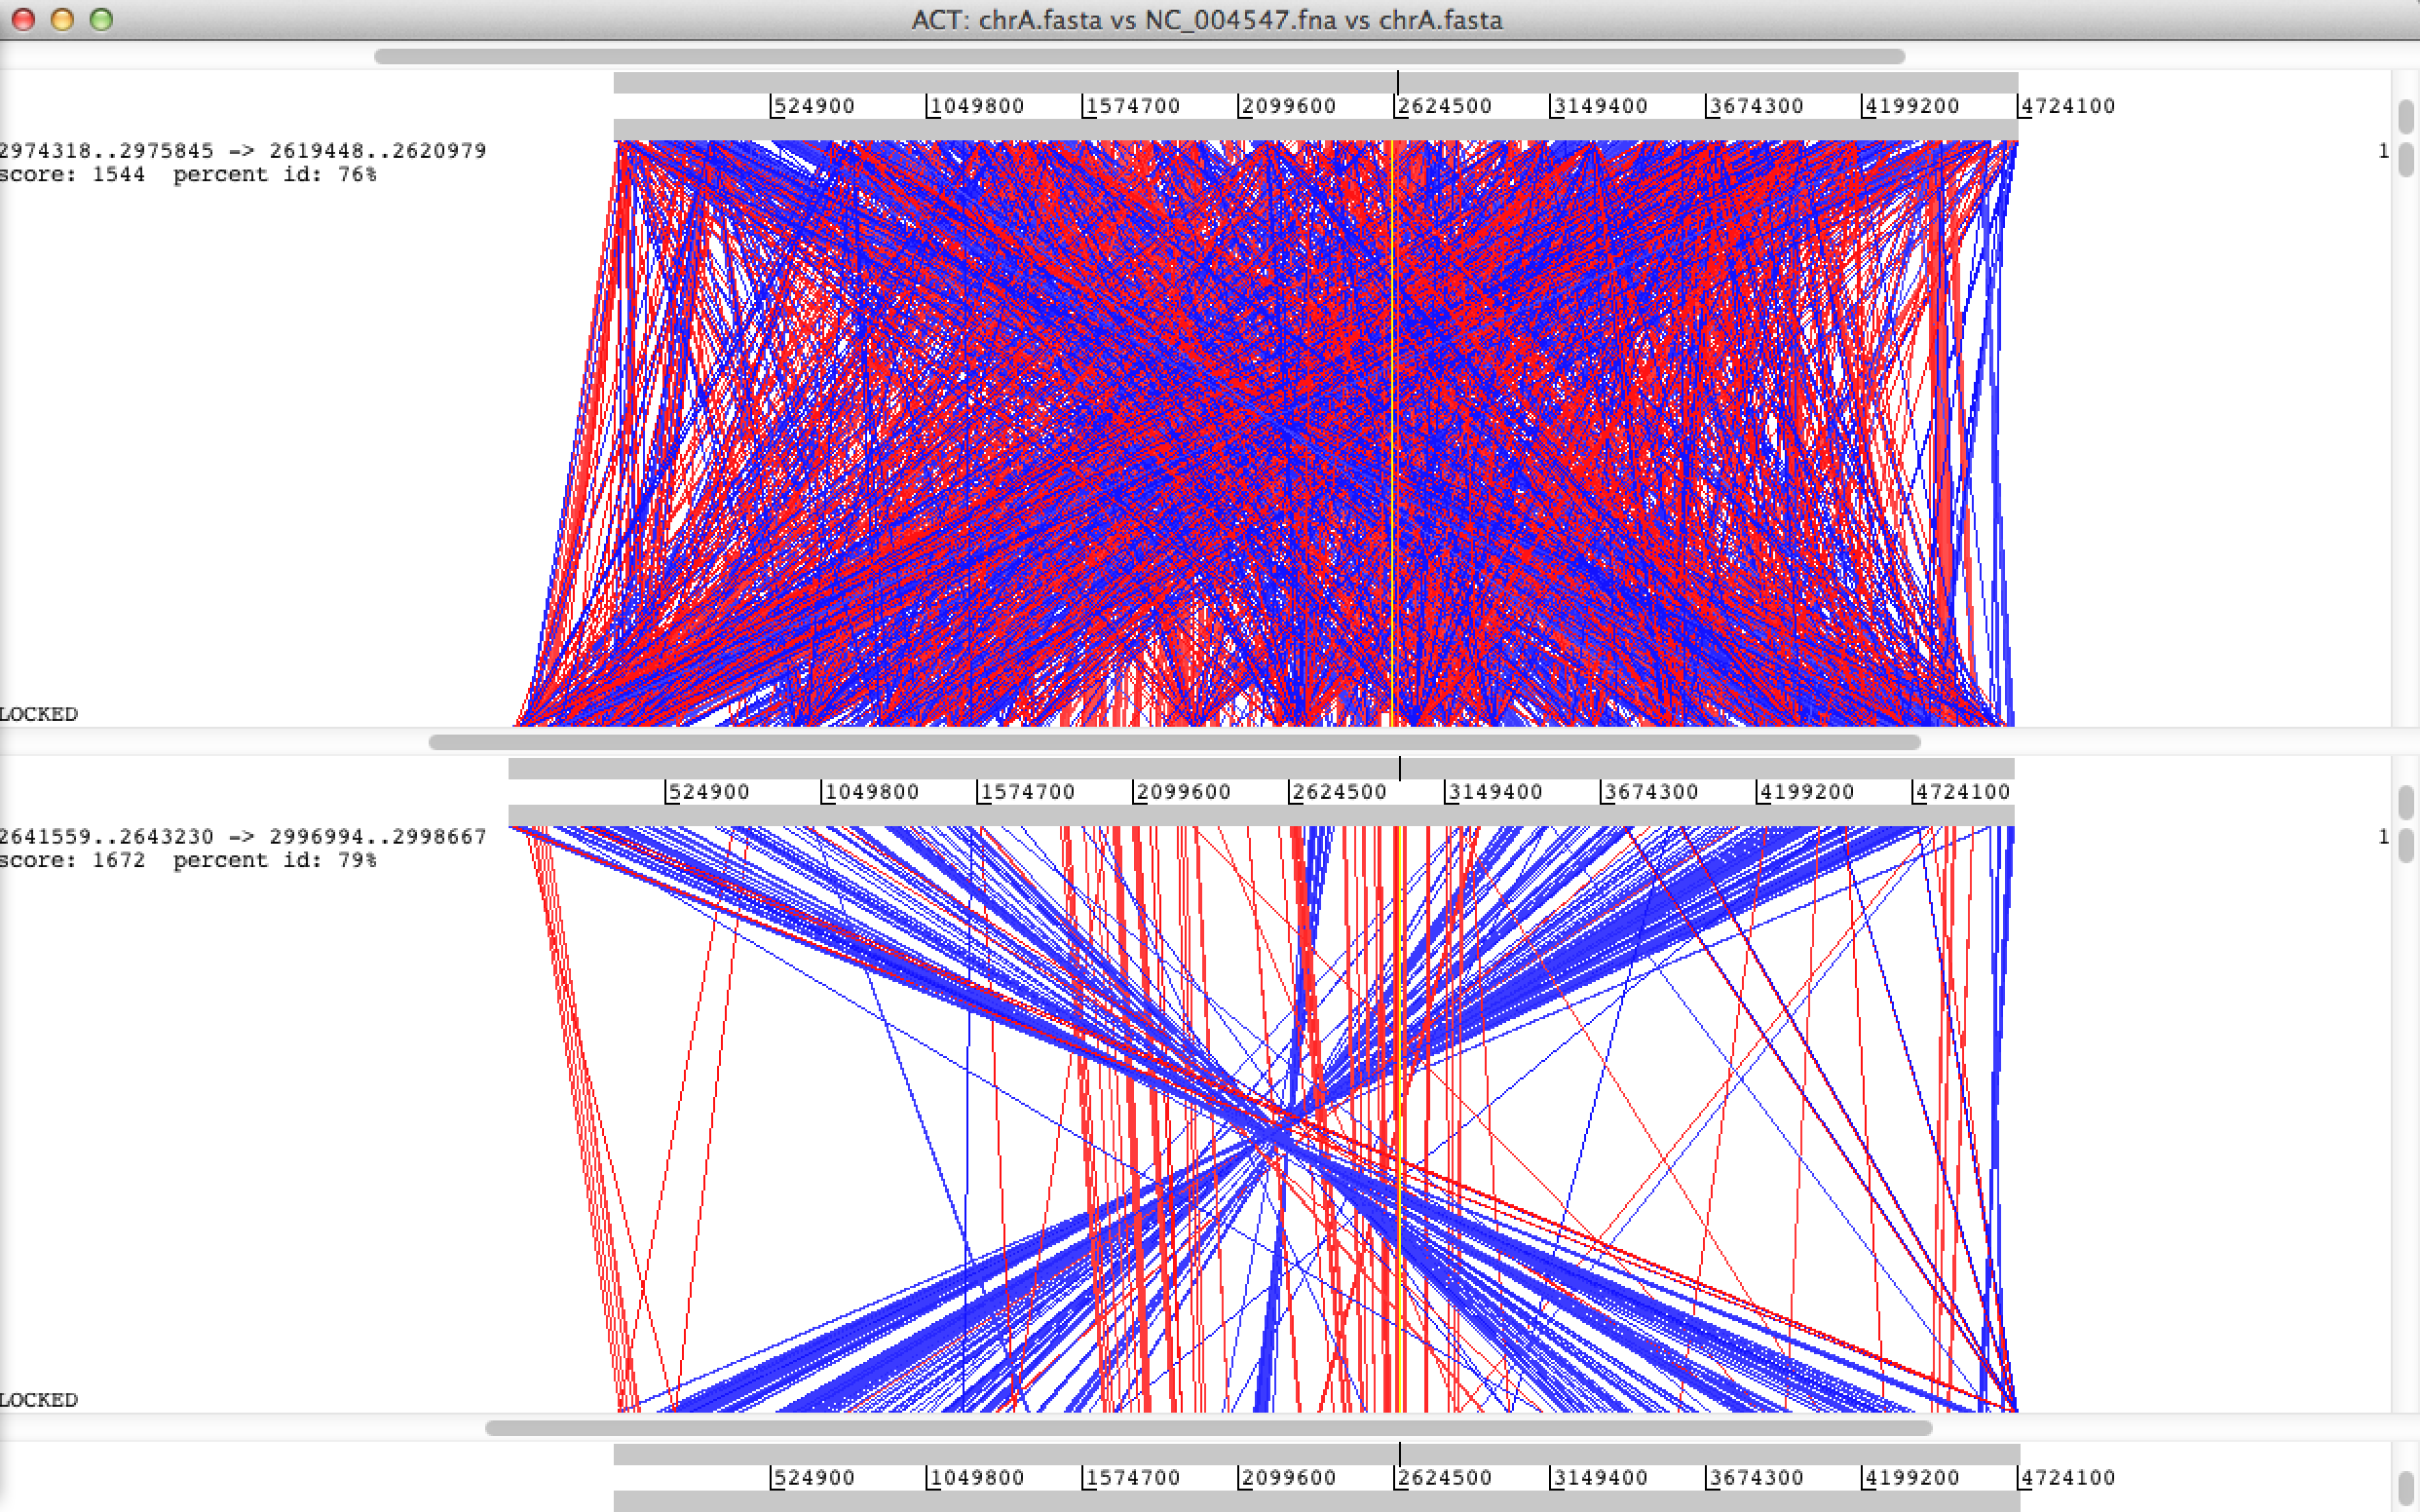
\includegraphics[width=0.9\textwidth]{images/act_wgs9}
  \end{center}    
\end{frame}

% BLAST vs megaBLAST
\begin{frame}
  \frametitle{MUMmer vs megaBLAST}
  Filter out weak BLAST matches - not quite identical:
  \begin{center}
    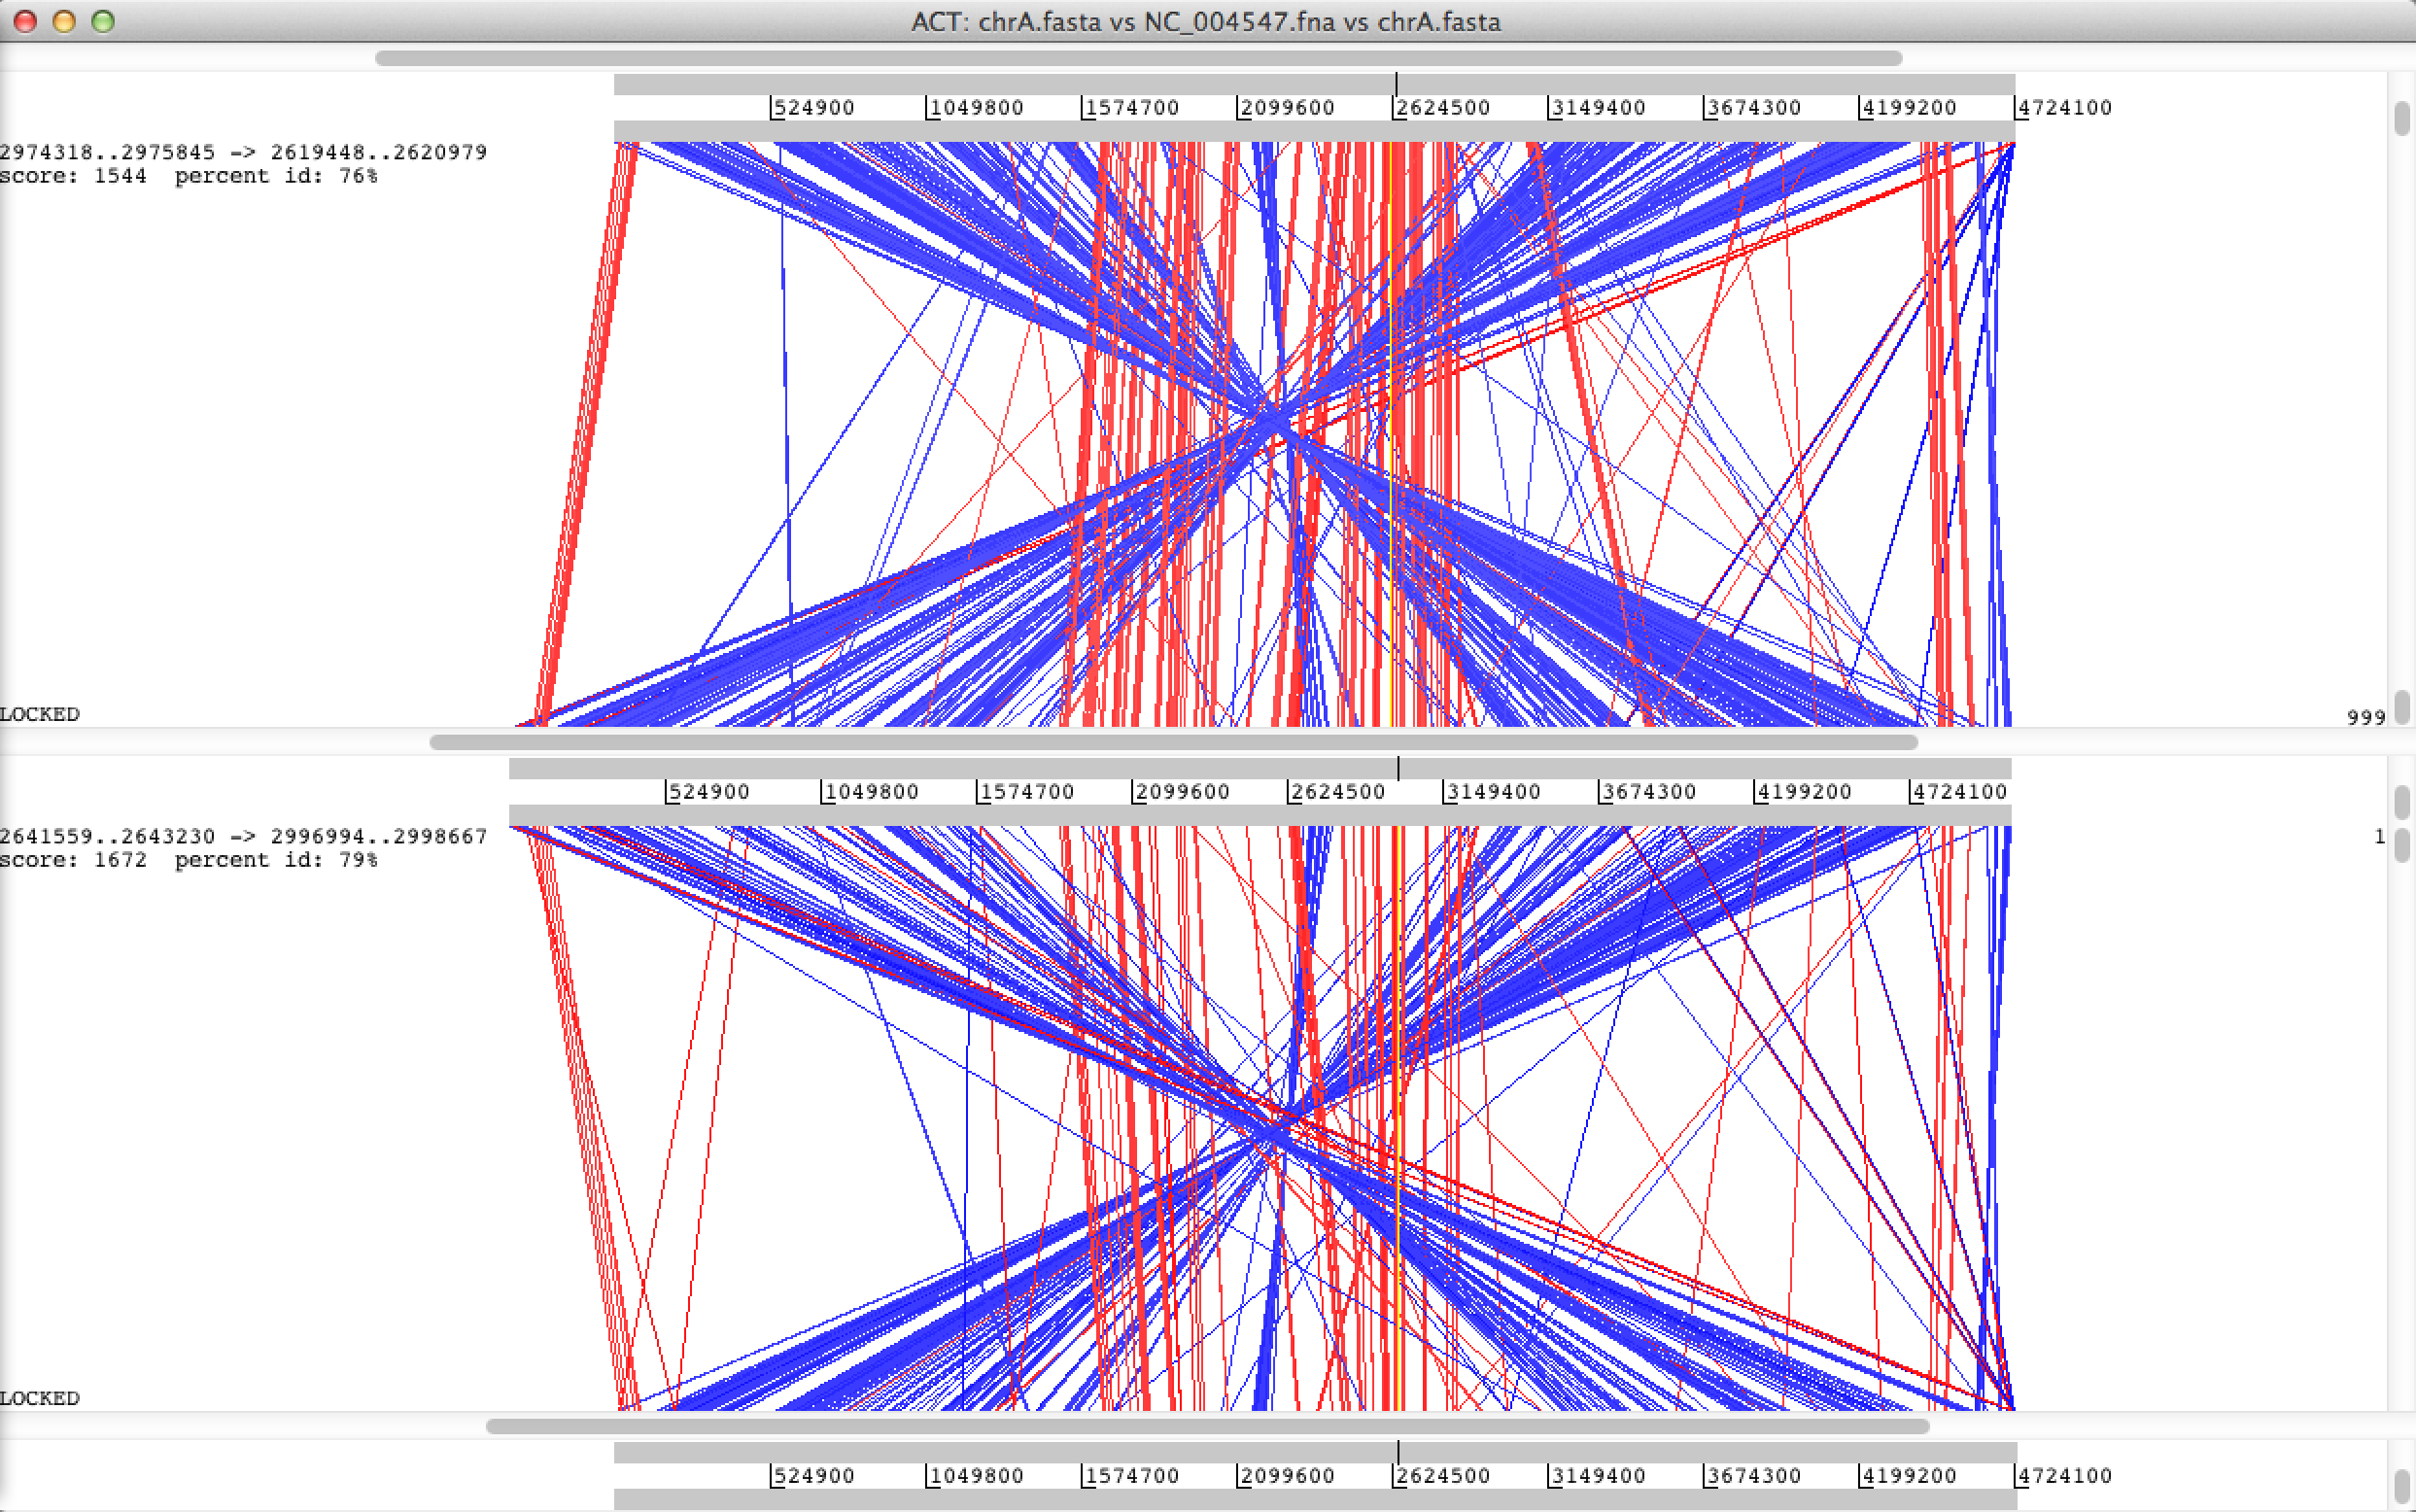
\includegraphics[width=0.9\textwidth]{images/act_wgs10}
  \end{center}    
\end{frame}

% SUBSECTION: Average Nucleotide Identity
\subsection{Average Nucleotide Identity}

% DNA-DNA hybridisation
\begin{frame}
  \frametitle{DNA-DNA hybridisation\footnote{\tiny{\href{http://dx.doi.org/10.1016/S0168-6445(00)00040-1}{Morello-Mora and Amann (2001) \textit{FEMS Micro. Rev.} \textbf{25}:39-67 doi:10.1016/S0168-6445(00)00040-1}}}}
  \begin{columns}[T]
    \begin{column}{5cm}
      \begin{itemize}
        \item Denature DNA from two organisms.
        \item Allow to anneal. Reassociation $\approx$ similarity, measured as $\Delta T$  of denaturation curves.
        \item ``Gold Standard'' for prokaryotic taxonomy, since 1960s. ``70\% identity $\approx$ same species.''
      \end{itemize}
    \end{column}
    \begin{column}{5cm}
      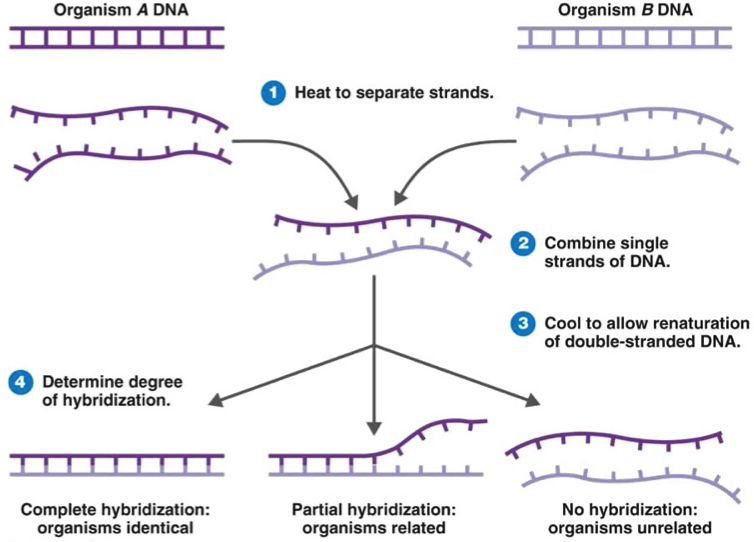
\includegraphics[width=1\textwidth]{images/ddh}
    \end{column}
  \end{columns}
  Proxy for sequence similarity - replace with genome analysis\footnote{\tiny{\href{http://dx.doi.org/10.1186/1471-2180-12-302}{Chan \textit{et al} (2012) \textit{BMC Microbiol.} \textbf{12}:302 doi:10.1186/1471-2180-12-302}}}?
\end{frame}

% ANIb
\begin{frame}
  \frametitle{Average Nucleotide Identity (ANIb)\footnote{\tiny{\href{http://dx.doi.org/10.1099/ijs.0.64483-0}{Goris \textit{et al}. (2007) \textit{Int. J. Syst. Biol.} \textbf{57}:81-91 doi:10.1099/ijs.0.64483-0}}}}
  \begin{columns}[T]
    \begin{column}{5cm}
      1. Break genomes into 1020t fragments\\
      2. \textbf{ANIb}: Mean \% identity of all BLASTN matches with $>30\%$ identity and $>70\%$ fragment coverage.\\[0.5cm]
      \begin{itemize}
        \item DDH:ANIb linear
        \item DDH:\%ID linear
        \item 70\%ID $\approx$ 95\%ANIb
      \end{itemize}
    \end{column}
    \begin{column}{5cm}
      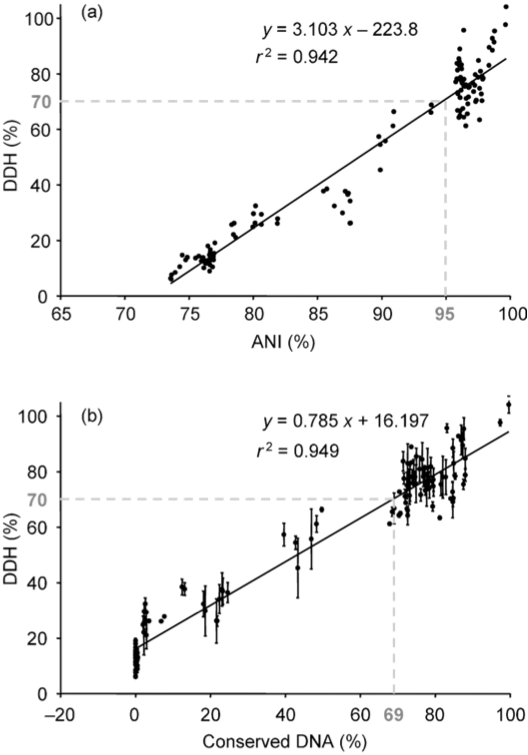
\includegraphics[width=1\textwidth]{images/ddh_ani_pid}
    \end{column}
  \end{columns}
\end{frame}

% ANIm
\begin{frame}
  \frametitle{Average Nucleotide Identity (ANIm)\footnote{\tiny{\href{http://dx.doi.org/10.1073/pnas.0906412106}{Richter and Rossello-Mora (2009) \textit{Proc. Natl. Acad. Sci. USA} \textbf{106}:19126-19131 doi:10.1073/pnas.0906412106}}}}
  \begin{columns}[T]
    \begin{column}{3cm}
      1. Align genomes (MUMmer)\\
      2. \textbf{ANIm}: Mean \% identity of all matches\\[0.25cm]
      \begin{itemize}
        \item DDH:ANIm linear
        \item 70\%ID $\approx$ 95\%ANIb
      \end{itemize}
    \end{column}
    \begin{column}{7cm}
      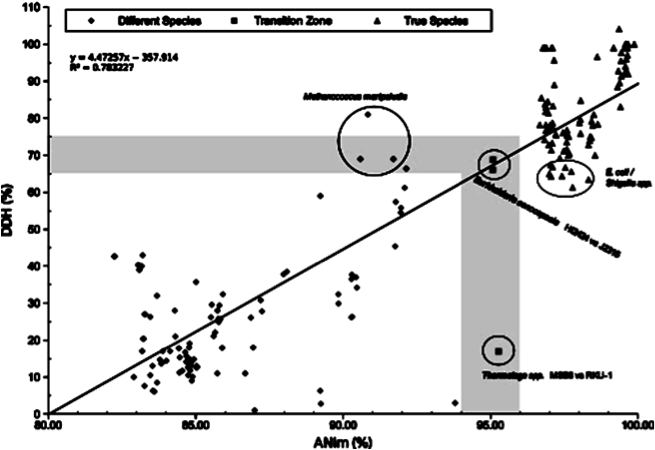
\includegraphics[width=1\textwidth]{images/ddh_anim}
    \end{column}
  \end{columns}
  \textbf{TETRA}: tetranucleotide frequency-based classifier introduced in same paper.
\end{frame}

% ANIb/ANIm/TETRA comparison
\begin{frame}
  \frametitle{ANI/TETRA comparison}
  All three methods applied to \textit{Anaplasma} spp.\\[0.25cm]
  \begin{columns}[T]
    \begin{column}{4cm}
    ANIb:\\
      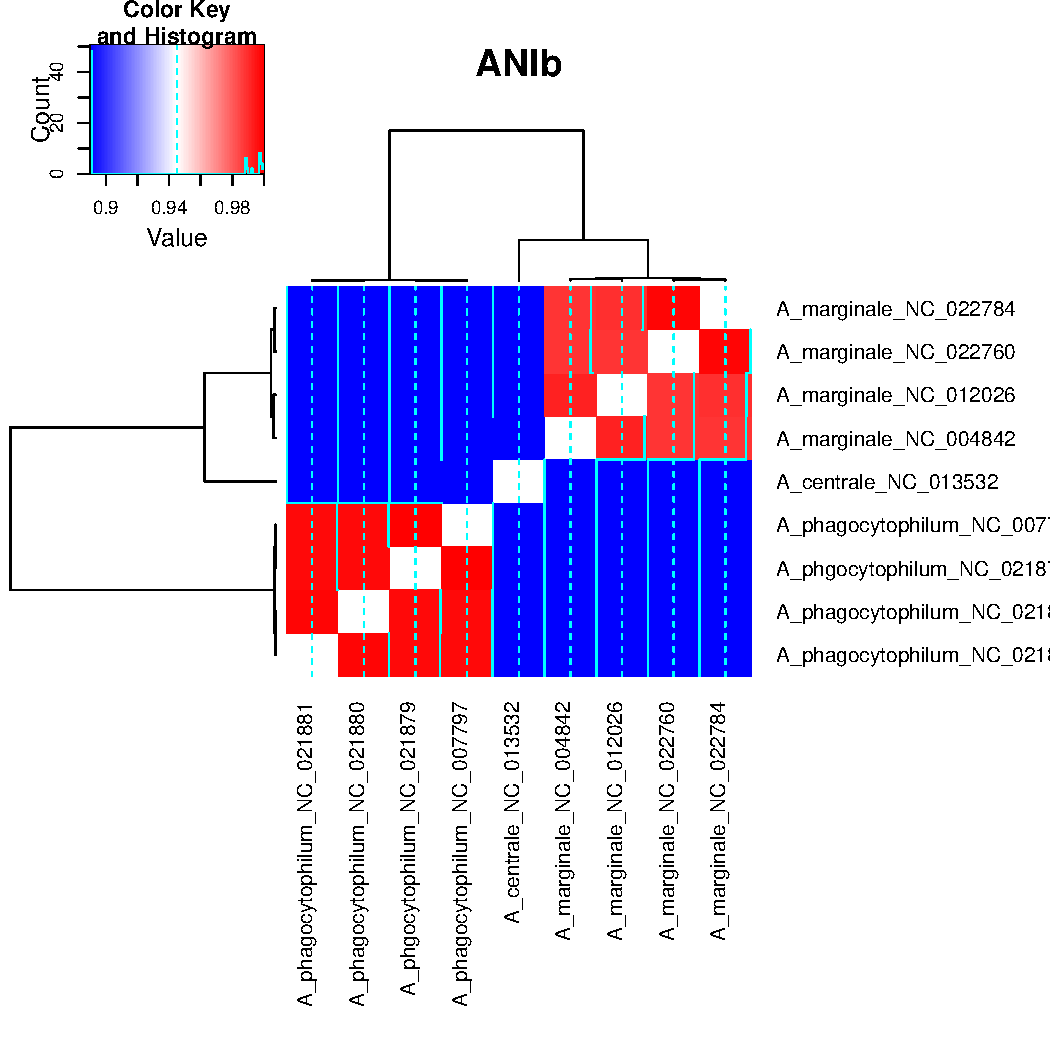
\includegraphics[width=1\textwidth]{images/ANIb}
    \end{column}
    \begin{column}{4cm}
    ANIm:\\
      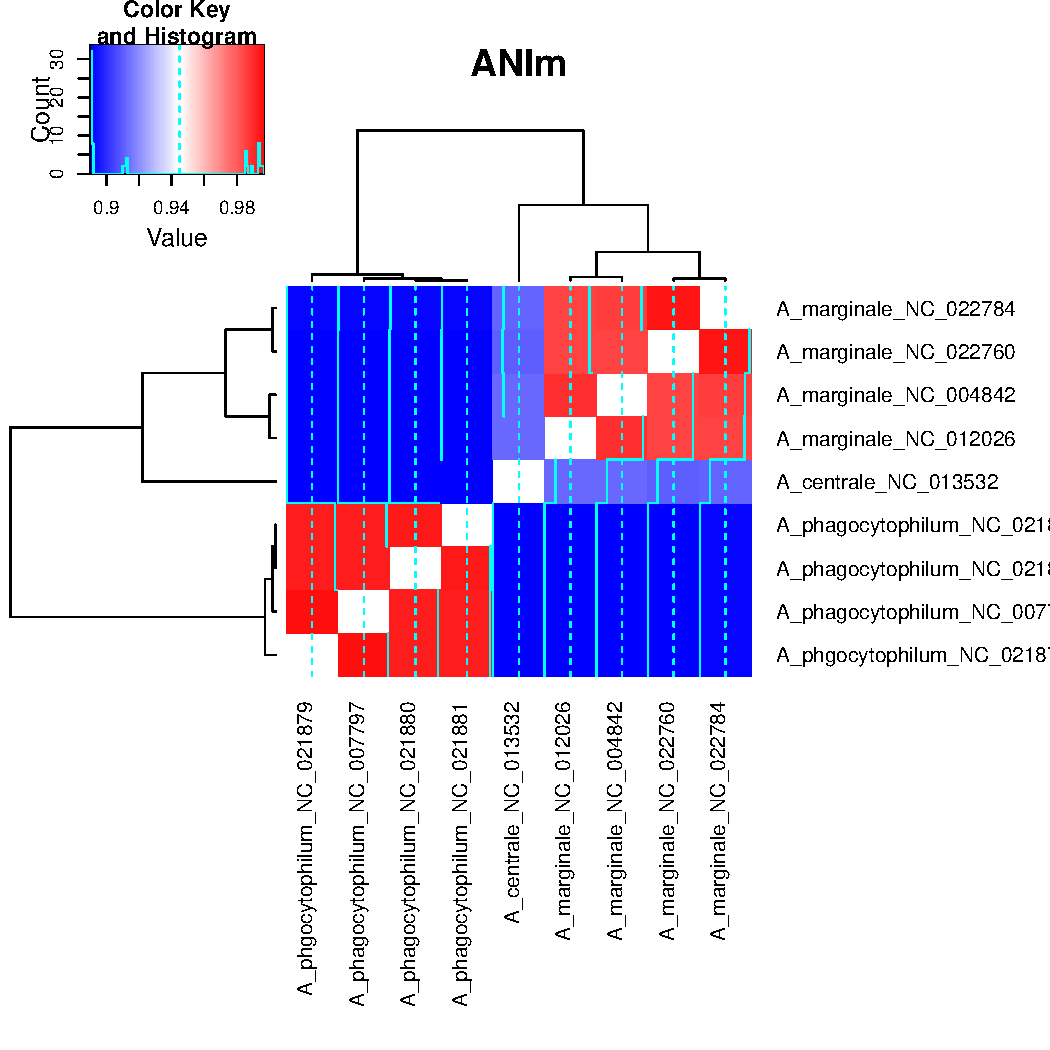
\includegraphics[width=1\textwidth]{images/ANIm}
    \end{column}
    \begin{column}{4cm}   
    TETRA:\\
      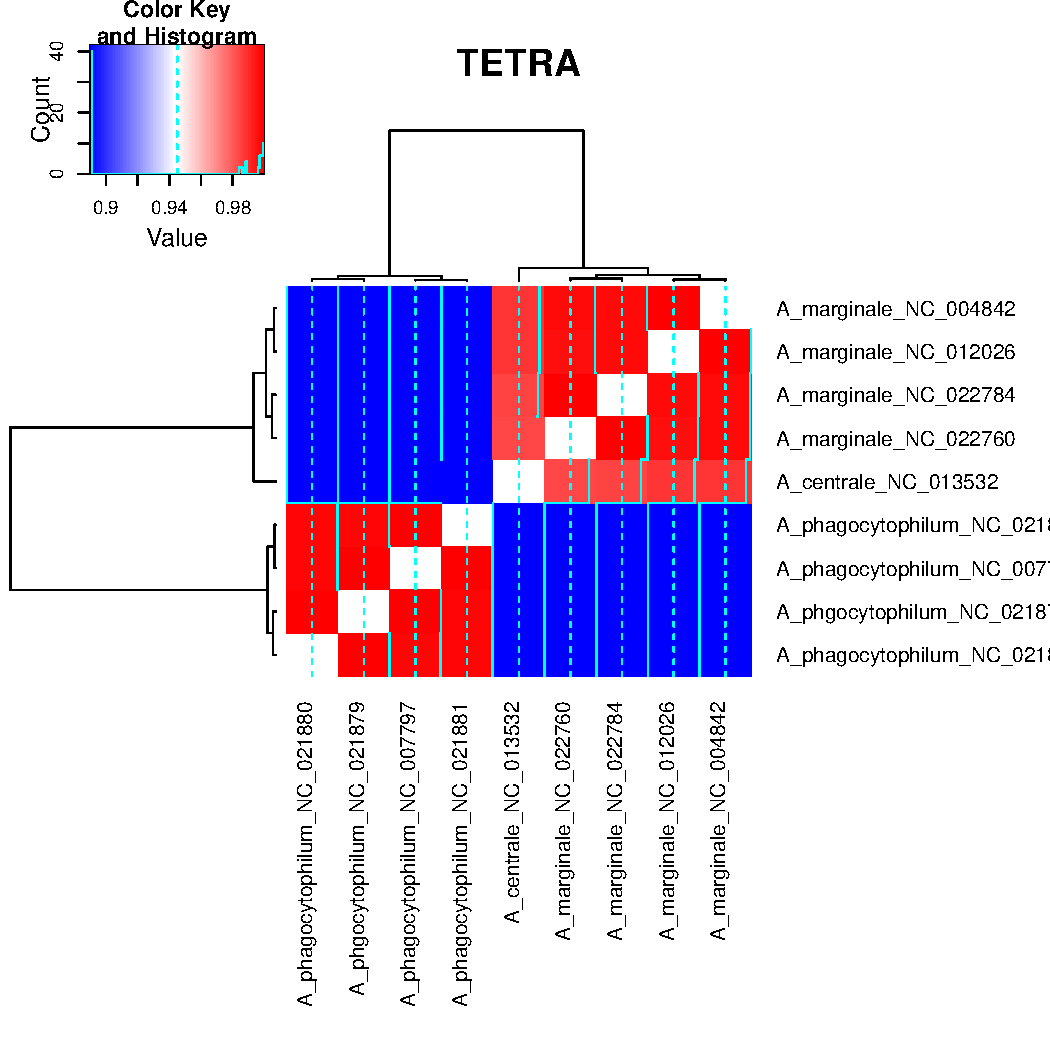
\includegraphics[width=1\textwidth]{images/TETRA}
    \end{column}
  \end{columns}       
  ANIb discards information, relative to ANIm: less sensitive\\
  ANIb/ANIm $\approx$ evolutionary history; TETRA $\approx$ bulk composition
\end{frame}

% ANIm in practice
\begin{frame}
  \frametitle{ANI in practice}
  Practical applications\footnote{\tiny{\href{http://dx.doi.org/10.1099/ijs.0.052944-0}{van der Wolf \textit{et al}. (2014) \textit{Int. J. Syst. Evol. Micr.} \textbf{64}:768-774 doi:10.1099/ijs.0.052944-0}}}\\[0.25cm]
  \begin{columns}[T]
    \begin{column}{5cm}
    29 \textit{Dickeya} isolates:\\
    species structure\\
      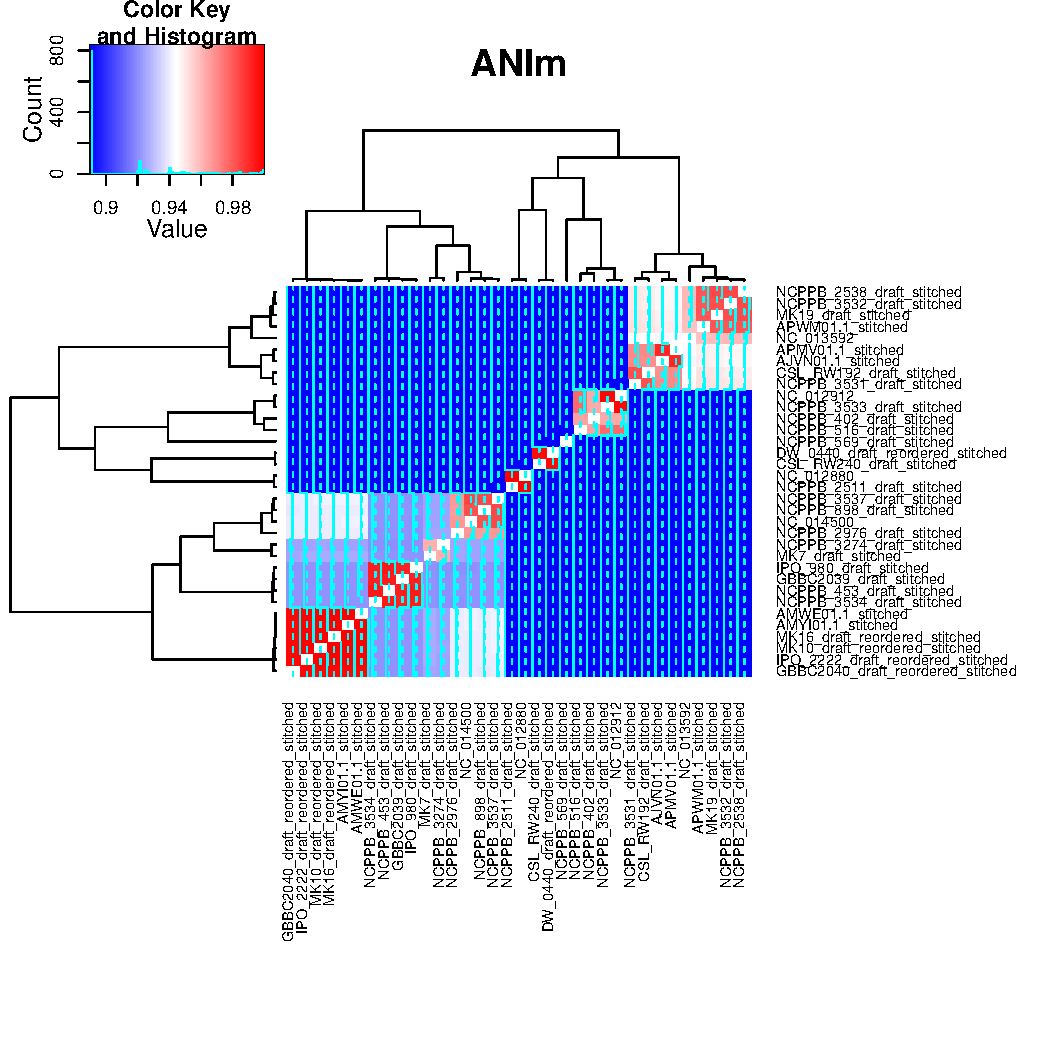
\includegraphics[width=1\textwidth]{images/ANIm_Dickeya}
    \end{column}
    \begin{column}{5cm}
    180 \textit{E.coli} isolates:\\
    subtyping
      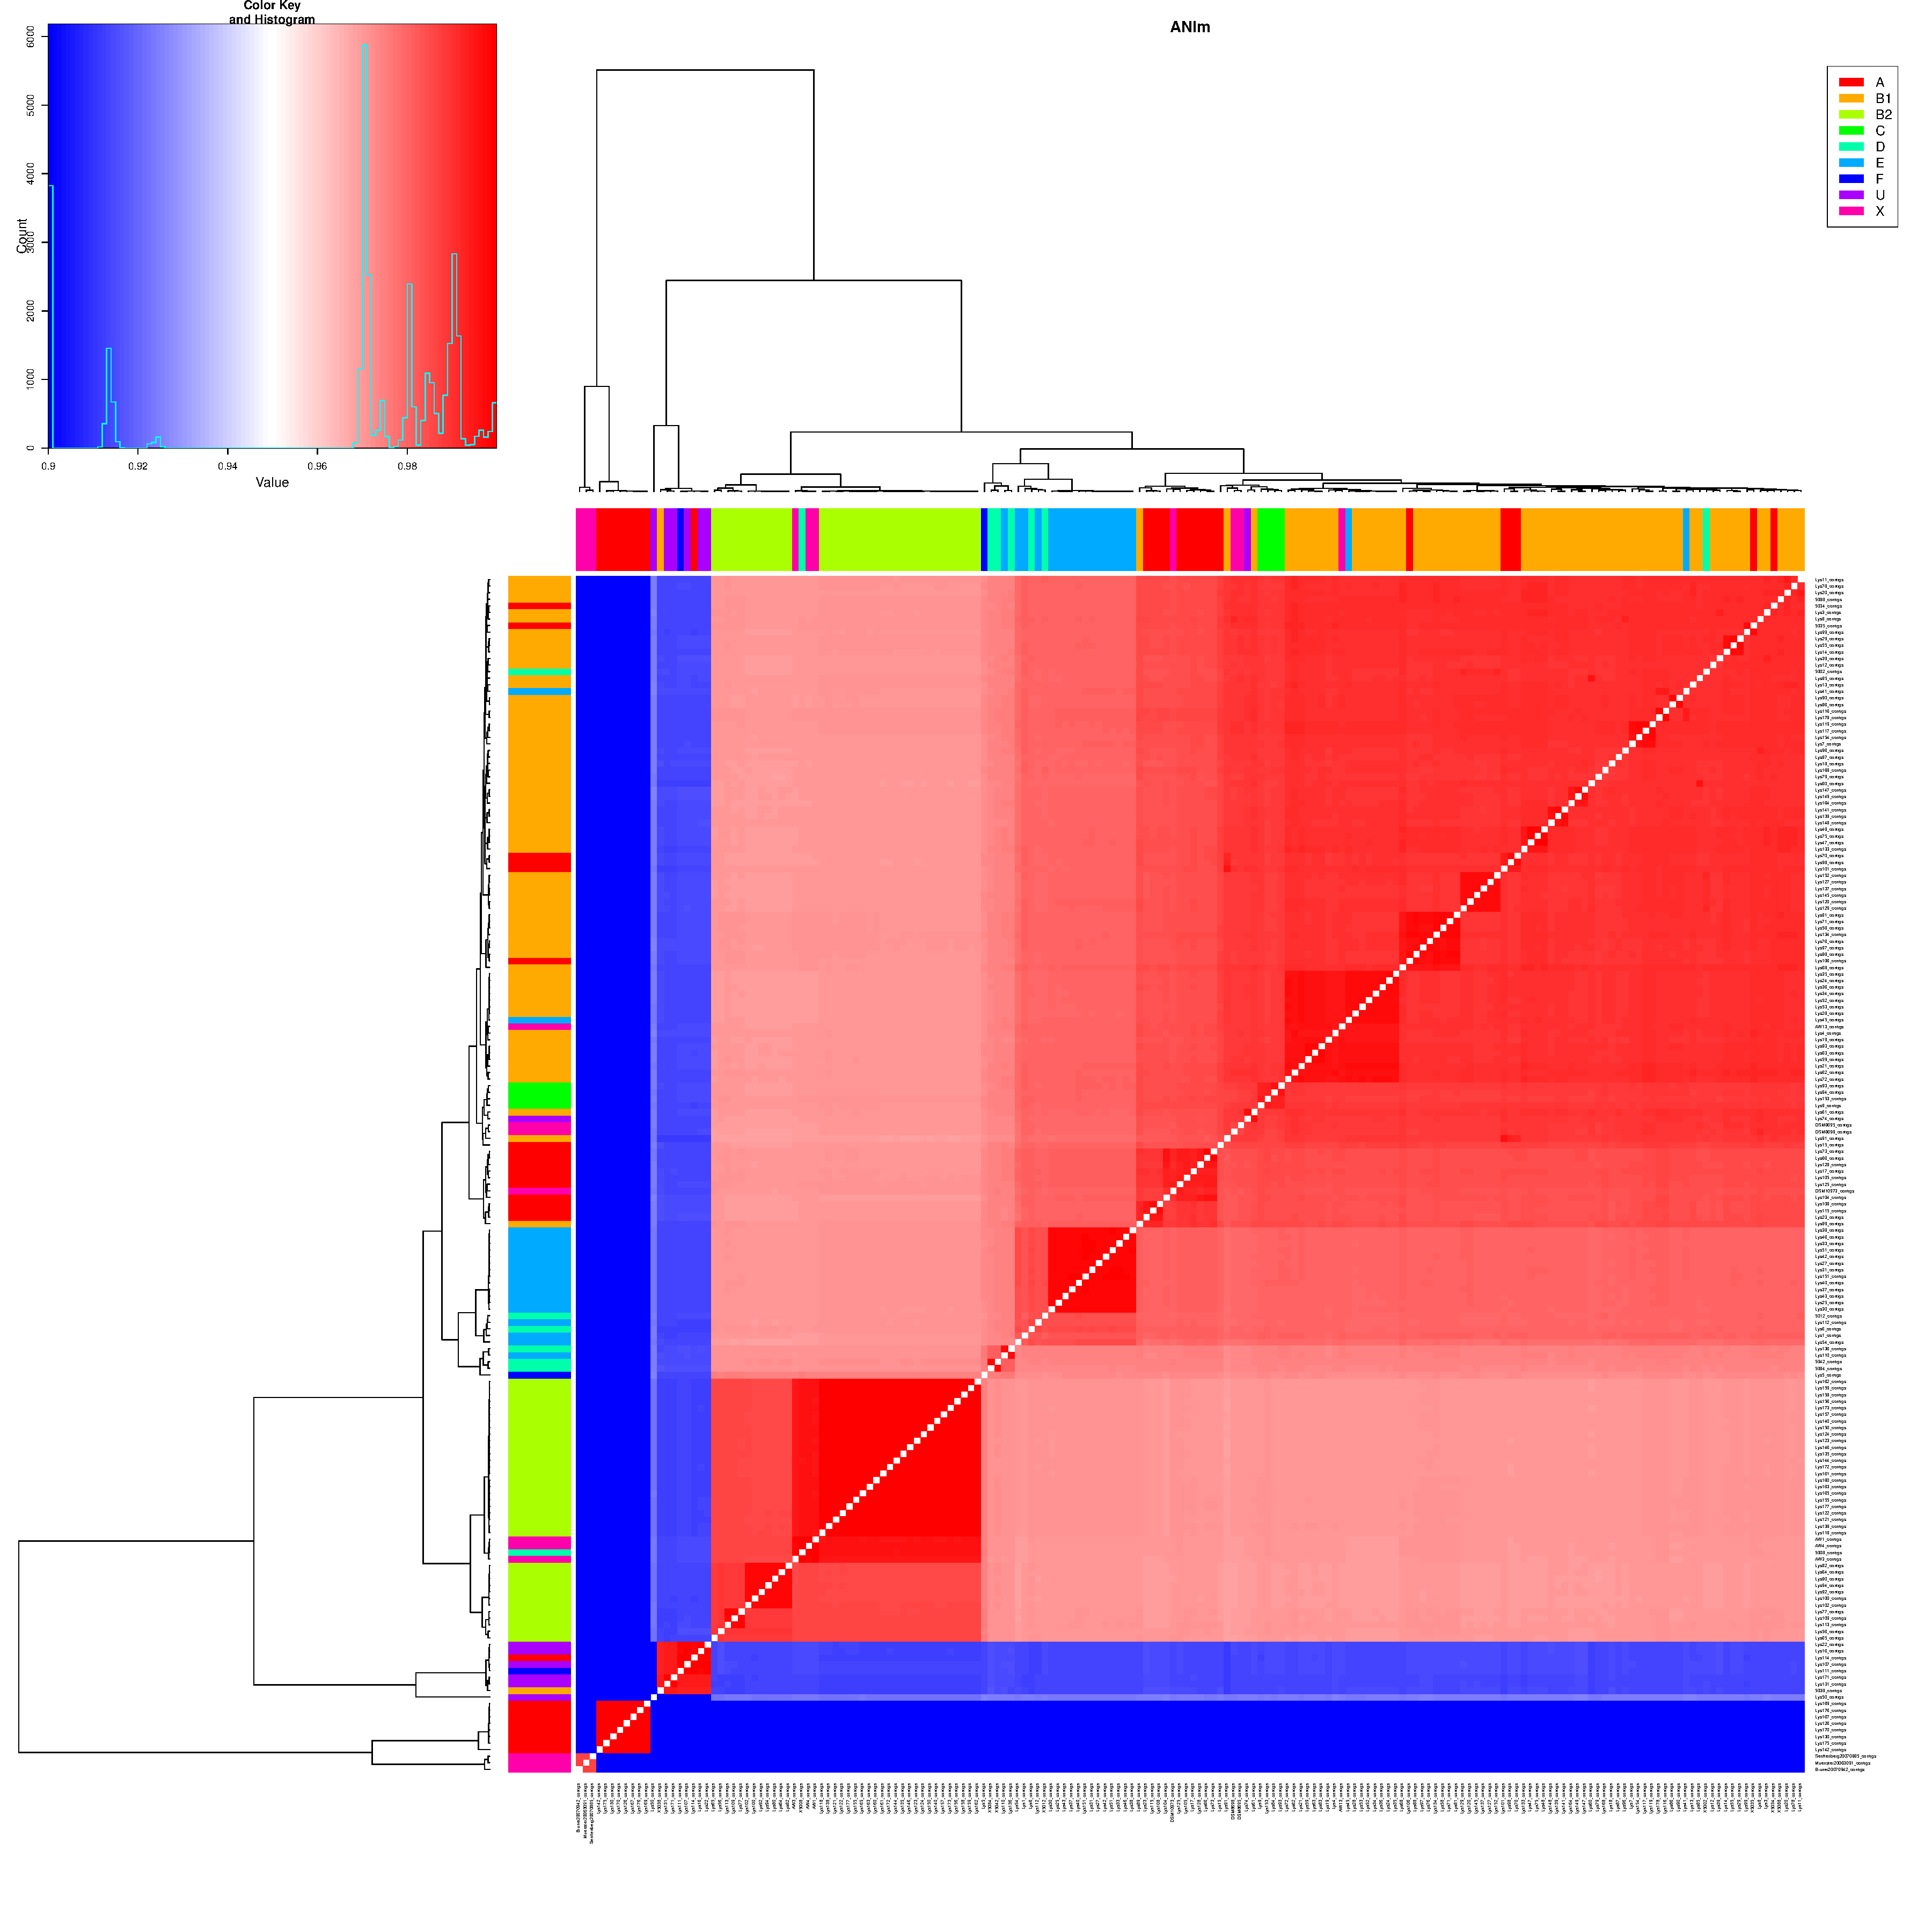
\includegraphics[width=1\textwidth]{images/ANIm_Ecoli}
    \end{column}
  \end{columns}       
\end{frame}

% SUBSECTION: Average Nucleotide Identity
\subsection{Whole Genome Alignment in Practice}

% Pyrococcus
\begin{frame}
  \frametitle{Collinearity and Synteny}
  Genome rearrangements occur, but there can still be conservation of sequence similarity and ordering.\\
  \begin{itemize}
    \item Two elements are \textbf{collinear} if they lie in the same linear sequence
    \item Two elements are \textbf{syntenous} (or \textit{syntenic}) if:
    \begin{itemize}
      \item (\textit{orig.}) they lie on the same chromosome
      \item (\textit{mod.}) there is conservation of blocks of order within the same chromosome
    \end{itemize}
  \end{itemize}    
  \textbf{Signs of evolutionary constraints, like sequence conservation or synteny, may indicate functional genome regions.}
\end{frame}

% Pyrococcus
\begin{frame}
  \frametitle{\textit{Pyrococcus} spp.\footnote{\tiny{\href{http://dx.doi.org/10.1093/nar/30.9.1902}{Zivanovic \textit{et al}. (2002) \textit{Nuc. Acids Res.} \textbf{30}:1902-1910 doi:10.1093/nar/30.9.1902}}}}
  Comparison of \textit{Pyrococcus} genomes (\textit{P. horikoshii}, \textit{P. abyssi}, \textit{P. furiosus}) shows chromosome-shuffling.\\
  \begin{center}
    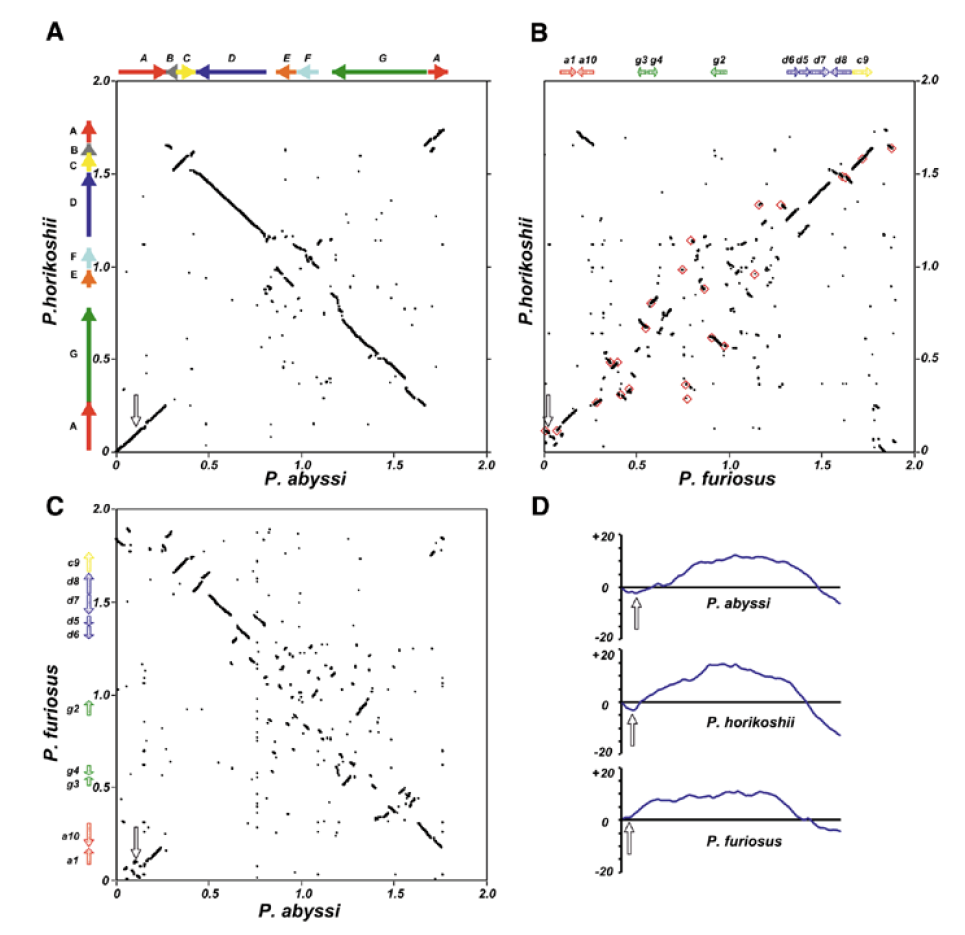
\includegraphics[height=0.65\textheight]{images/pyrococcus}
  \end{center}    
\end{frame}

\begin{frame}
  \frametitle{\textit{Pyrococcus} spp.\footnote{\tiny{\href{http://dx.doi.org/10.1093/nar/30.9.1902}{Zivanovic \textit{et al}. (2002) \textit{Nuc. Acids Res.} \textbf{30}:1902-1910 doi:10.1093/nar/30.9.1902}}}}
  Comparison of \textit{Pyrococcus} genomes (\textit{P. horikoshii}, \textit{P. abyssi}, \textit{P. furiosus}) shows chromosome-shuffling.\\[0.2cm]
  Three types of rearrangement:
  \begin{enumerate}
    \item inversion and translation across the replication axis
    \item inversion and translocation restricted to a replichore (`one side' of axis)
    \item mobility of long clusters of repeat sequences
  \end{enumerate}  
  Transposition was a major cause of genomic disruption  
\end{frame}

% Vibrio mimicus
\begin{frame}
  \frametitle{\textit{Vibrio mimicus} \footnote{\tiny{\href{http://dx.doi.org/10.1073/pnas.1013825107}{Hasan \textit{et al}. (2010) \textit{Proc. Natl. Acad. Sci. USA} \textbf{107}:21134-21139 doi:10.1073/pnas.1013825107}}}}
  Chromosome C-II carries genes associated with environmental adaptation; C-I carries virulence genes.\\
  C-II has undergone extensive rearrangement; C-I has not.\\
  \begin{center}
    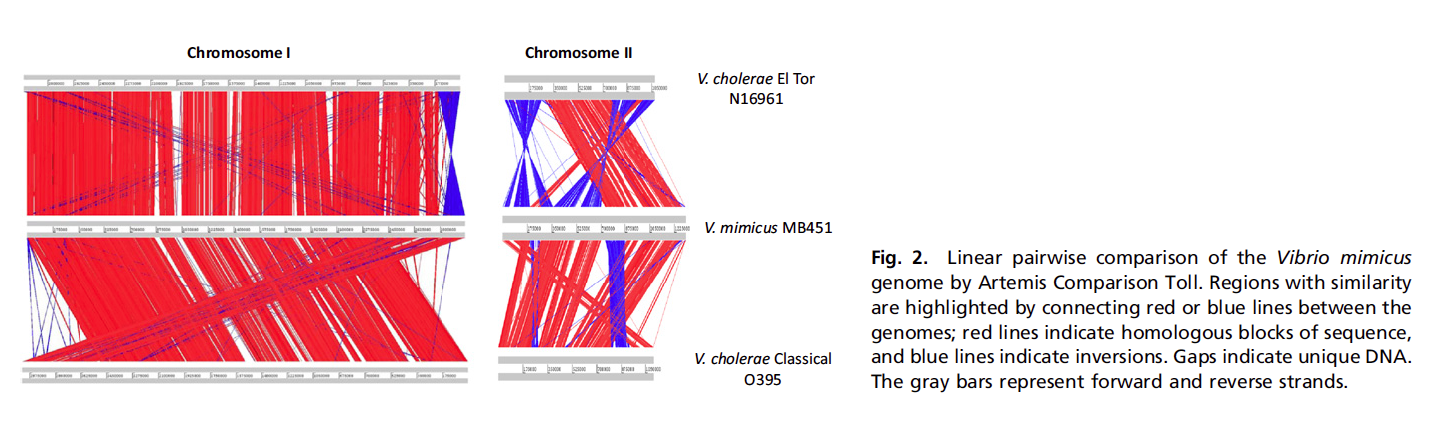
\includegraphics[width=1\textwidth]{images/v_mimicus}
  \end{center}    
  Suggests modularity of genome organisation, and mechanisms for virulence adaptation.
\end{frame}

% Serratia symbiotica
\begin{frame}
  \frametitle{\textit{Serratia symbiotica} \footnote{\tiny{\href{http://dx.doi.org/10.1093/gbe/evr002}{Burke and Moran (2011) \textit{Genome Biol. Evol.} \textbf{3}:195-208 doi:10.1093/gbe/evr002}}}}
  \textit{S. symbiotica} is a recently evolved symbiont of aphids\\
  Massive genomic decay is an adaptation to the new environment.\\
  \begin{center}
    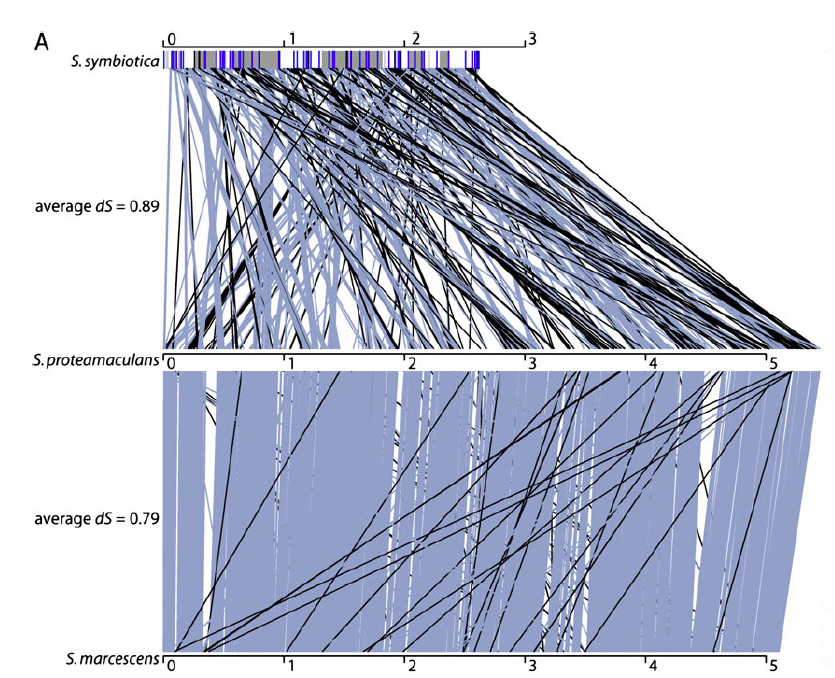
\includegraphics[width=0.75\textheight]{images/s_symbiotica}
  \end{center}    
\end{frame}

% SUBSECTION: Average Nucleotide Identity
\subsection{Ordering Draft Genomes By Alignment}

% Multiple genome alignment
\begin{frame}
  \frametitle{Multiple genome alignment is hard}
  Really, really hard.\\[0.2cm]
  Analogous to problems with multiple sequence alignment (three or more sequences).
  \begin{itemize}
    \item Computationally extremely expensive ($O(L^n)$, $L$=length of sequence, $n$=number of sequences) 
    \item NP-complete problem: no known efficient way to find a solution
  \end{itemize}
  Heuristic (approximate) methods are used, most commonly:
  \begin{itemize}
    \item Progressive alignment
    \item Iterative alignment
  \end{itemize}
\end{frame}

% Mauve
\begin{frame}
  \frametitle{Mauve\footnote{\tiny{\href{http://dx.doi.org/10.1101/gr.2289704}{Darling \textit{et al}. (2004) \textit{Genome Res.} \textbf{14}:1394-1403 doi:10.1101/gr.2289704}}}}
  Progressive alignment tool, with a GUI. Application to nine enterobacteria: rearrangement of homologous backbone.
  \begin{center}
    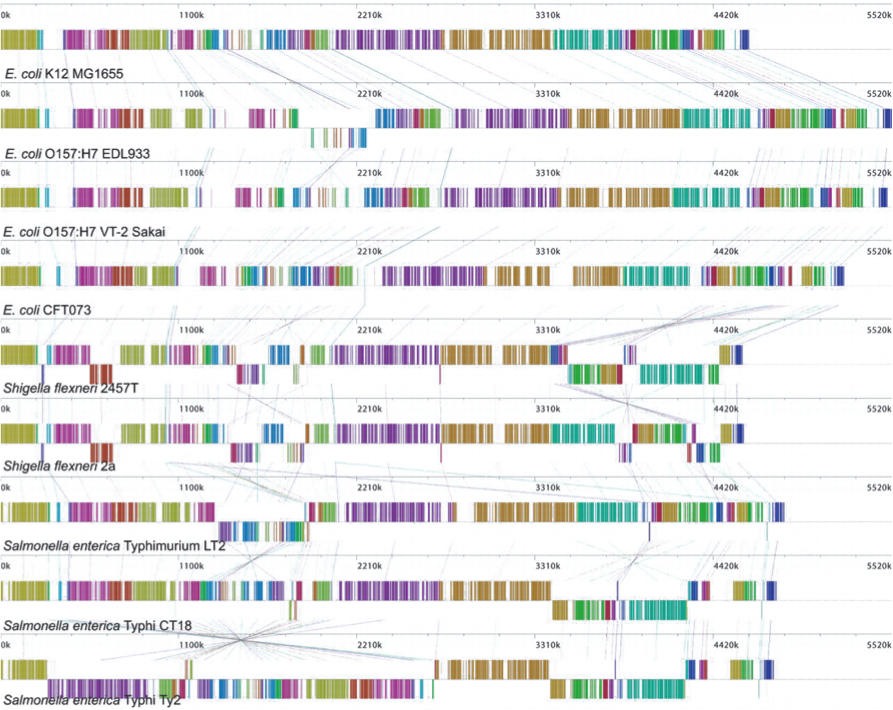
\includegraphics[height=0.46\textheight]{images/mauve_entero}
  \end{center}        
  Alternatives include MLAGAN\footnote{\tiny{\href{http://dx.doi.org/10.1101/gr.926603}{Brudno \textit{et al}. (2003) \textit{Genome Res.} \textbf{13}:721-731 doi:10.1101/gr.926603}}} and MUMmer\footnote{\tiny{\href{http://dx.doi.org/10.1186/gb-2004-5-2-r12}{Kurtz \textit{et al}. (2004) \textit{Genome Biol.} \textbf{5}:R12 doi:10.1186/gb-2004-5-2-r12}}}
\end{frame}

% The Mauve algorithm
\begin{frame}
  \frametitle{Mauve algorithm\footnote{\tiny{\href{http://dx.doi.org/10.1101/gr.2289704}{Darling \textit{et al}. (2004) \textit{Genome Res.} \textbf{14}:1394-1403 doi:10.1101/gr.2289704}}}}
  \begin{columns}[T]
    \begin{column}{5cm}
      \begin{enumerate}
        \item Find local alignments (\textit{multi-MUMs})
        \item Build guide tree from multi-MUMs
        \item Select subset of multi-MUMs as anchors, and partition into Local Collinear Blocks (LCBs): consistently ordered subsets
        \item Progressive alignment against guide tree
      \end{enumerate}
    \end{column}
    \begin{column}{5cm}
      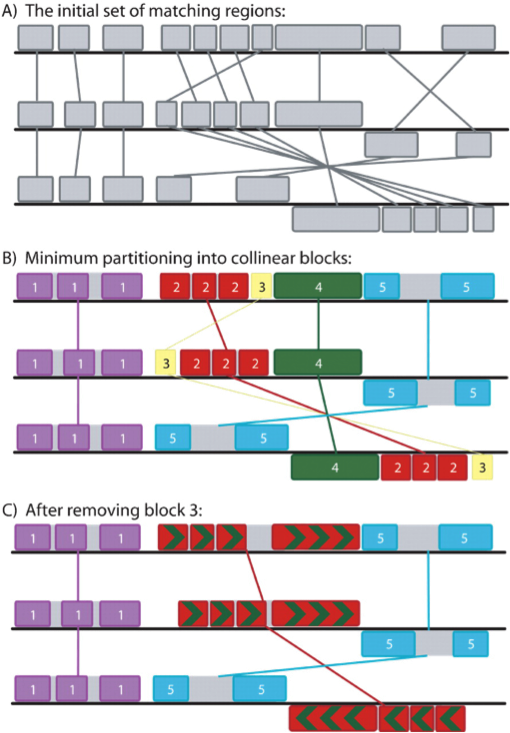
\includegraphics[width=1\textwidth]{images/mauve_algorithm}
    \end{column}
  \end{columns}
\end{frame}

% Reordering contigs
\begin{frame}
  \frametitle{Reordering contigs\footnote{\tiny{\href{http://dx.doi.org/10.1101/gr.2289704}{Darling \textit{et al}. (2004) \textit{Genome Res.} \textbf{14}:1394-1403 doi:10.1101/gr.2289704}}}}
  Mauve also enables draft genome reordering.\\
  Once LCBs are identified, can apply Mauve Contig Mover to reorder contigs
  \begin{center}
    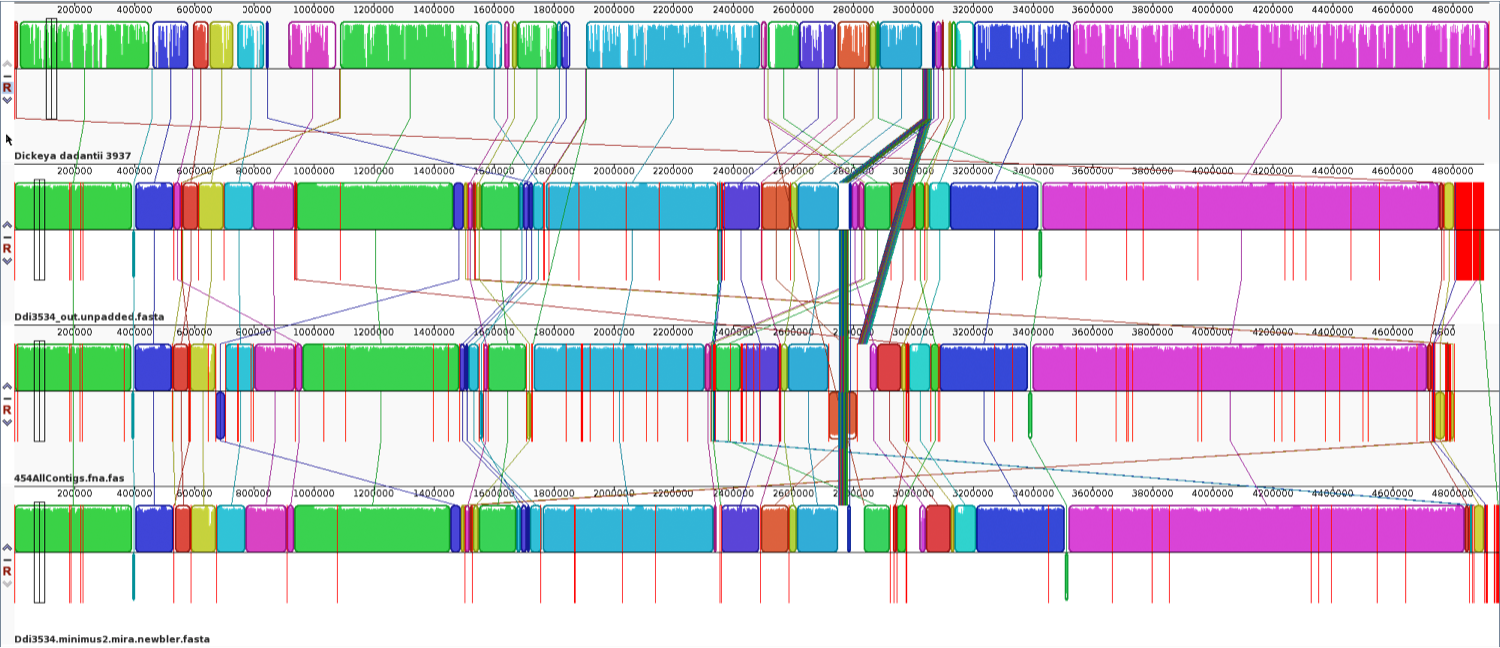
\includegraphics[width=0.9\textwidth]{images/mauve_dickeya}
  \end{center}    
  Example exercise in \url{data/whole_genome_alignment}
\end{frame}


% SUBSECTION: Average Nucleotide Identity
\subsection{Chromosome painting}

% DNA-DNA hybridisation
\begin{frame}
  \frametitle{Chromosome painting\footnote{\tiny{\href{http://dx.doi.org/10.1093/molbev/mst055}{Yahara \textit{et al}. (2013) \textit{Mol. Biol. Evol.} \textbf{30}:1454-1464 doi:10.1093/molbev/mst055}}}}
  ``Chromosome painting'' infers recombination-derived `chunks'\\
  Genome's haplotype constructed in terms of recombination events from a `donor' to a `recipient'\\
  \begin{center}
    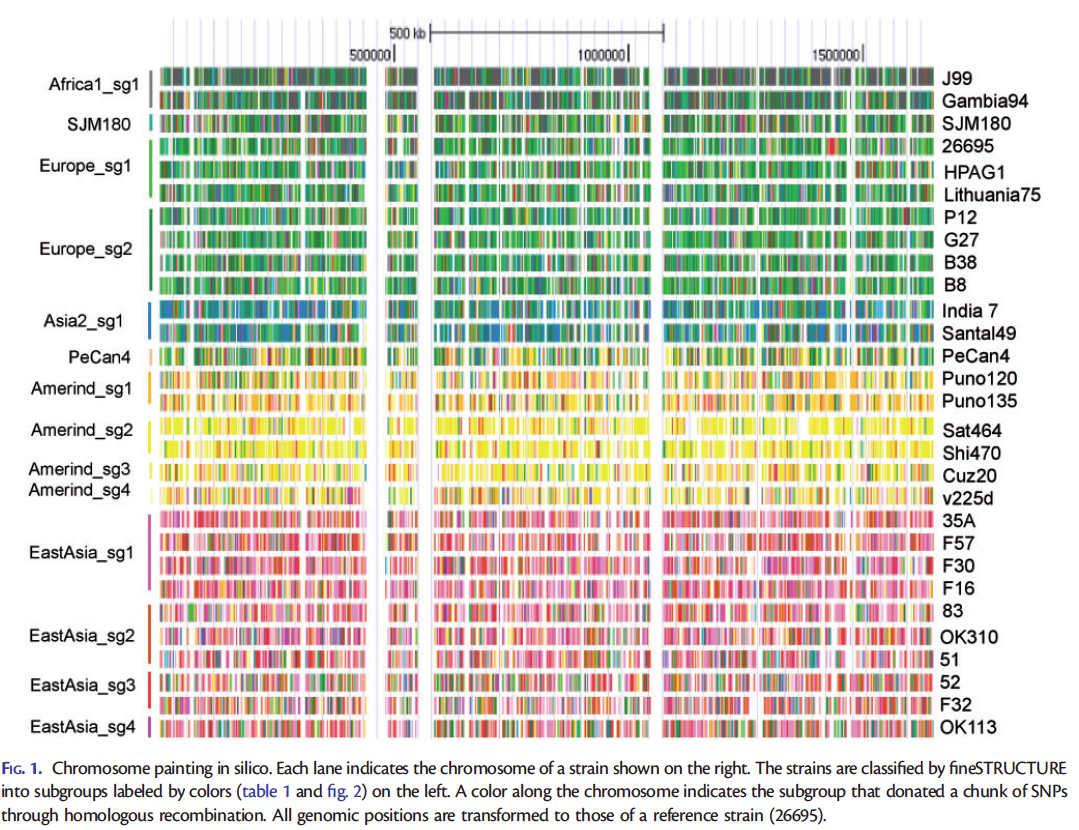
\includegraphics[width=0.7\textwidth]{images/chromosome_painting}
  \end{center}     
\end{frame}

% DNA-DNA hybridisation
\begin{frame}
  \frametitle{Chromosome painting\footnote{\tiny{\href{http://dx.doi.org/10.1093/molbev/mst055}{Yahara \textit{et al}. (2013) \textit{Mol. Biol. Evol.} \textbf{30}:1454-1464 doi:10.1093/molbev/mst055}}}}
  Recombination events summarised in a \textit{coancestry matrix}.\\
  In \textit{H. pylori}, most recombination is within geographical bounds, but there is asymmetrical donation from Amerind to European isolates.
  \begin{center}
    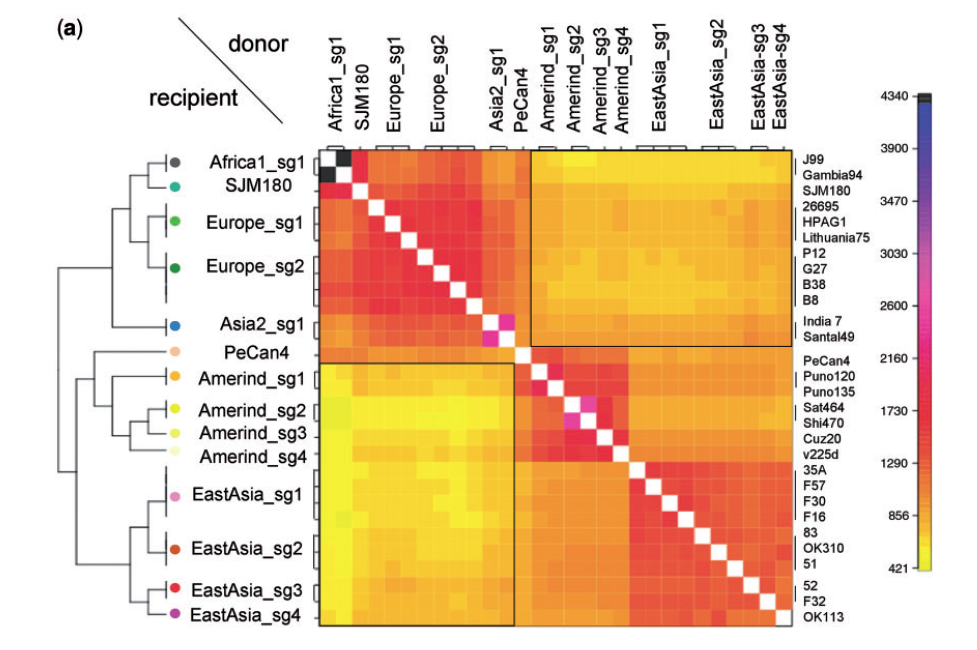
\includegraphics[width=0.75\textwidth]{images/coancestry}
  \end{center}     
\end{frame}